% !TeX program = xelatex
% =====================================================================
% 2026 高教社杯全国大学生数学建模竞赛 A 题《药材的烘干问题》论文
%
% 编译要求：官方 LaTeX 模板类 cumcmthesis.cls（可在国赛官网或 Overleaf
% 官方模板获取），用 XeLaTeX 编译两遍：
%     xelatex main.tex && xelatex main.tex
% 论文表格由 results/tables/paper_table*.csv 自动生成：
%     python paper/build_tables.py
% =====================================================================
\documentclass[withoutpreface,bwprint]{cumcmthesis}

\usepackage{booktabs}
\usepackage{longtable}
\usepackage{array}
\usepackage{listings}
\usepackage{xcolor}
\setmonofont{Noto Sans Mono}

% 图按章节编号；题目指定的表 1--6 仍保留原编号。
\makeatletter
\@addtoreset{figure}{section}
\renewcommand{\thefigure}{\arabic{section}-\arabic{figure}}
\makeatother

% 代码附录样式
\lstset{
  basicstyle=\ttfamily\footnotesize,
  breaklines=true,
  columns=fullflexible,
  frame=single,
  numbers=left,
  numberstyle=\tiny\color{gray},
  showstringspaces=false,
  keywordstyle=\color{blue!70!black},
  commentstyle=\color{green!45!black},
}

% ---------------- 基本信息（提交前填写） ----------------
\title{药材烘干过程的热湿耦合数值模拟}
\tihao{A}
\baominghao{XXXXXXXXX}     % TODO: 报名号
\schoolname{XX大学}         % TODO: 学校全称
\membera{队员一} \memberb{队员二} \memberc{队员三}  % TODO: 三名队员姓名
\supervisor{指导教师}       % TODO: 指导教师姓名

\begin{document}

\maketitle

% ==================== 摘要 ====================
\begin{abstract}
  本文研究圆柱形药材在时变热风中的预热、降速干燥和失水收缩过程。以干基
  含水率 $X$ 与温度 $T$ 为状态变量，在固定半径域和材料坐标域分别建立
  一维轴对称热湿耦合方程；用单元中心有限体积法、Backward Euler 启动和
  变步长 BDF2 推进，并以连续事件函数确定终止时间。该路线将附件环境、
  实测半径、正式工作簿和独立验证串联为可复现的计算链。

  针对问题一的初始强边界层，采用附录 2 常物性模型，令 $N=2561$、
  初始最大步长 $0.03125\ \mathrm{s}$，以分辨表面水分的快速变化。计算得
  $t=1800\ \mathrm{s}$ 时，表面温度为 $36.7856\ ^\circ\mathrm{C}$，
  表面含水率为 $1.5102\ \mathrm{kg\,kg^{-1}}$；中心含水率仍为
  $2.5500\ \mathrm{kg\,kg^{-1}}$，定量呈现热扩散快于水分扩散的阶段差异。
  该分辨率由 $t=1\ \mathrm{s}$ 表面含水率的空间、时间加密试验确定，避免
  将极薄表层梯度平滑为非物理的体平均变化。

  针对问题二的长时非线性场，采用附录 3 的
  $\rho(X),c_p(X),k(X),D_{\mathrm{eff}}(X,\Theta)$，在每个时间层以
  Picard 迭代冻结并更新物性，界面系数取调和平均，表面 Robin 条件按
  半单元扩散阻力与对流阻力串联离散。$3\ \mathrm{h}$ 时中心和表面含水率
  分别为 $1.7662$、$1.0081\ \mathrm{kg\,kg^{-1}}$，而对应温度为
  $49.85$、$49.97\ ^\circ\mathrm{C}$，说明后续过程主要受内部水分迁移控制。
  环境输入在前 $4\ \mathrm{h}$ 采用附件 1 的分段线性插值，此后固定为
  $50.165\ ^\circ\mathrm{C}$ 和 $0.04986\ \mathrm{kg\,kg^{-1}}$；附录 3、4
  未给出新对流系数，故 $h_T,h_m$ 沿用题设值并纳入灵敏度分析，而不额外拟合
  未观测参数。

  针对问题三，将全域约束写为
  $g(t)=\max_rX(r,t)-0.15$，在相邻时间层出现符号跨越后以二分法定位，
  不将规则 $60\ \mathrm{s}$ 输出网格误作事件精度。固定半径正式计算给出
  $t_{\mathrm{dry}}=205885.5\ \mathrm{s}=57.1904\ \mathrm{h}$；终止时
  中心含水率为 $0.1500\ \mathrm{kg\,kg^{-1}}$，表面为 $0.0525\ \mathrm{kg\,kg^{-1}}$。

  针对问题四，利用 PCHIP 对附件 2 的 $R(t)$ 保形插值，在
  $\xi=r/R(t)$ 上求解附录 4 物性模型，并将固定物理坐标的越界位置输出为空。
  实测收缩联合情景下得到 $t_{\mathrm{dry}}=182964.7\ \mathrm{s}=50.8235\ \mathrm{h}$；
  同物性固定半径反事实为 $129.11\ \mathrm{h}$，表明缩短扩散路径是收缩
  加速的解释性因素。方法要点是将半单元 Robin 阻力、连续事件定位和实测
  移动域统一于同一求解器。Bessel/Duhamel 基准、网格收敛和时间步收敛共同
  验证：最大步长由 $60$ 降至 $15\ \mathrm{s}$ 时，两工况终止时间仅变化
  $0.26$ 和 $0.12\ \mathrm{s}$。灵敏度分析中 $h_m$ 减半使终止时间延长
  $7.45\ \mathrm{h}$；在 $48$--$52\ ^\circ\mathrm{C}$ 范围内，$52\ ^\circ\mathrm{C}$
  将终止时间缩短 $3.1962\ \mathrm{h}$（$5.59\%$），终点均匀性变化小于
  网格可辨识水平，故仅称其为考察区间内的优选温度；模型未含品质降解与设备
  能耗机制，不将该端点外推为实际生产的全局最优。

  \keywords{热湿耦合 \quad 圆柱药材 \quad 有限体积法 \quad 移动域模型 \quad 事件定位}
\end{abstract}

% ==================== 一、问题重述 ====================
\section{问题重述}

药材热风烘干问题可归结为一维轴对称非稳态热湿传递初边值问题，以及在其
场解上的连续事件定位。已知圆柱介质的几何尺寸（半径 $R_0=0.02\ \mathrm{m}$、
长度 $L=0.25\ \mathrm{m}$）、初始状态（温度 $T_0=28\ ^\circ\mathrm{C}$、
干基含水率 $X_0=2.55\ \mathrm{kg\,kg^{-1}}$）、烘房环境的时变序列
$T_a(t),\chi_a(t)$ 与实测半径轨迹 $R(t)$，需以径向温度 $T(r,t)$ 与干基
含水率 $X(r,t)$ 为状态量，在径向域内依次求解下列四个递进的定解问题；
各问的物性关系分别取自题目附录 2--4
\cite{simal1998,mujumdar2014,cumcm2026}。

\begin{figure}[htbp]
  \centering
  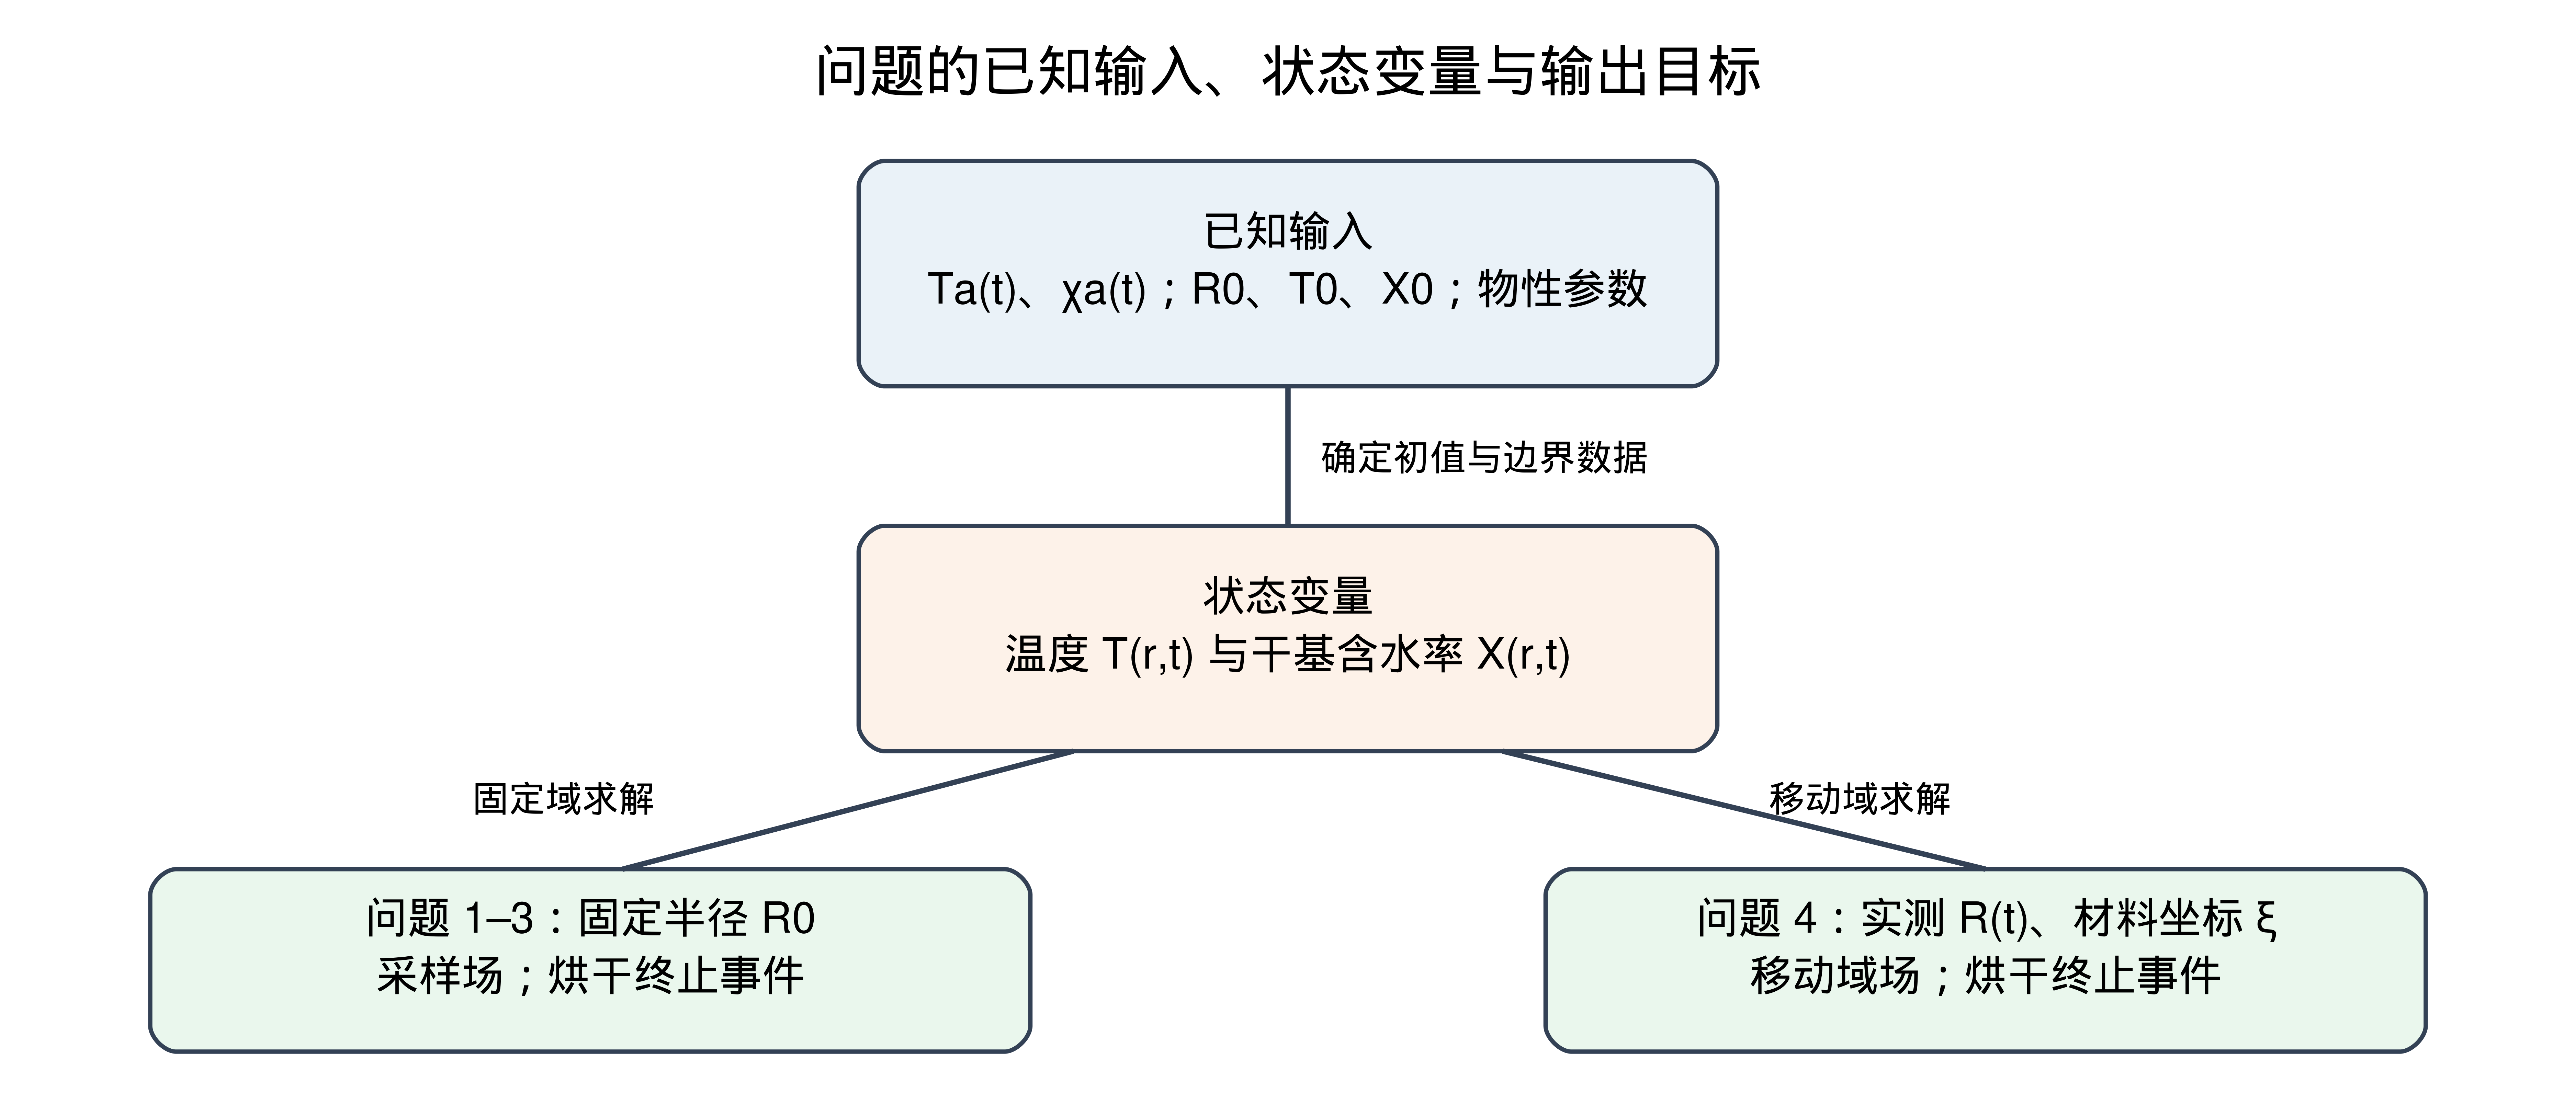
\includegraphics[width=0.86\linewidth]{figures/problem_restatement_relation}
  \caption{问题的已知输入、状态变量与输出目标关系}
  \label{fig:problem-restatement-relation}
\end{figure}

\begin{itemize}
  \item \textbf{问题一（预热阶段场演化）。}在常物性及固定半径 $R_0$ 下，
  求解 $t\in[0,1800\ \mathrm{s}]$ 内的径向温度场 $T(r,t)$ 与水分场
  $X(r,t)$。
  \item \textbf{问题二（变物性固定域场演化）。}保持 $R_0$ 不变，引入随
  $(T,X)$ 动态变化的耦合热物性与有效扩散系数，求解 $t\in[0,3\ \mathrm{h}]$
  内的非线性热湿演化场。
  \item \textbf{问题三（连续烘干终止事件定位）。}在变物性固定域模型基础上，
  求解全域含水率满足连续不等式约束
  $\max_{0\le r\le R_0}X(r,t)\le0.15\ \mathrm{kg\,kg^{-1}}$ 的首次穿越时刻
  $t_{\mathrm{dry}}$。
  \item \textbf{问题四（失水收缩移动域演化）。}引入实测半径轨迹 $R(t)$，
  在移动几何域 $r\in[0,R(t)]$ 下重求烘干终止时刻 $t_{\mathrm{dry}}$，
  并评估几何收缩对内部传质路径的影响。
\end{itemize}

% ==================== 二、问题分析 ====================
\section{问题分析}

四问并非彼此独立的计算任务，而是沿“短时固定域场--长时非线性场--
全域终止事件--实测收缩移动域”逐层增加时间尺度、物性非线性、约束类型
与几何条件的同一热湿传递问题。药材长径比为 $25/4\approx6.25$，端面总
面积仅约为侧面积的 $8\%$；结合周向边界近似均匀，采用一维轴对称径向
描述可保留主导梯度\cite{hussain2003}。四问的共同未知量为温度 $T(r,t)$
与干基含水率 $X(r,t)$；附件 1 的 $T_a(t),\chi_a(t)$ 经 Robin 边界进入
模型，而附录物性将二者参数耦合。以下按【数学本质】【状态与约束】
【求解难点与拟用算法】三层分别剖析。

图 \ref{fig:route} 将本地输入、四问模型链、数值算法、约束输出与独立校验
连接为一条可追溯路线：实线表示数据流与计算流；虚线表示将主求解器输出的
定型结果送入后置独立校验与情景分析模块，从而保持前向计算链的单向闭环与
后置验证的独立性。

\begin{figure}[htbp]
  \centering
  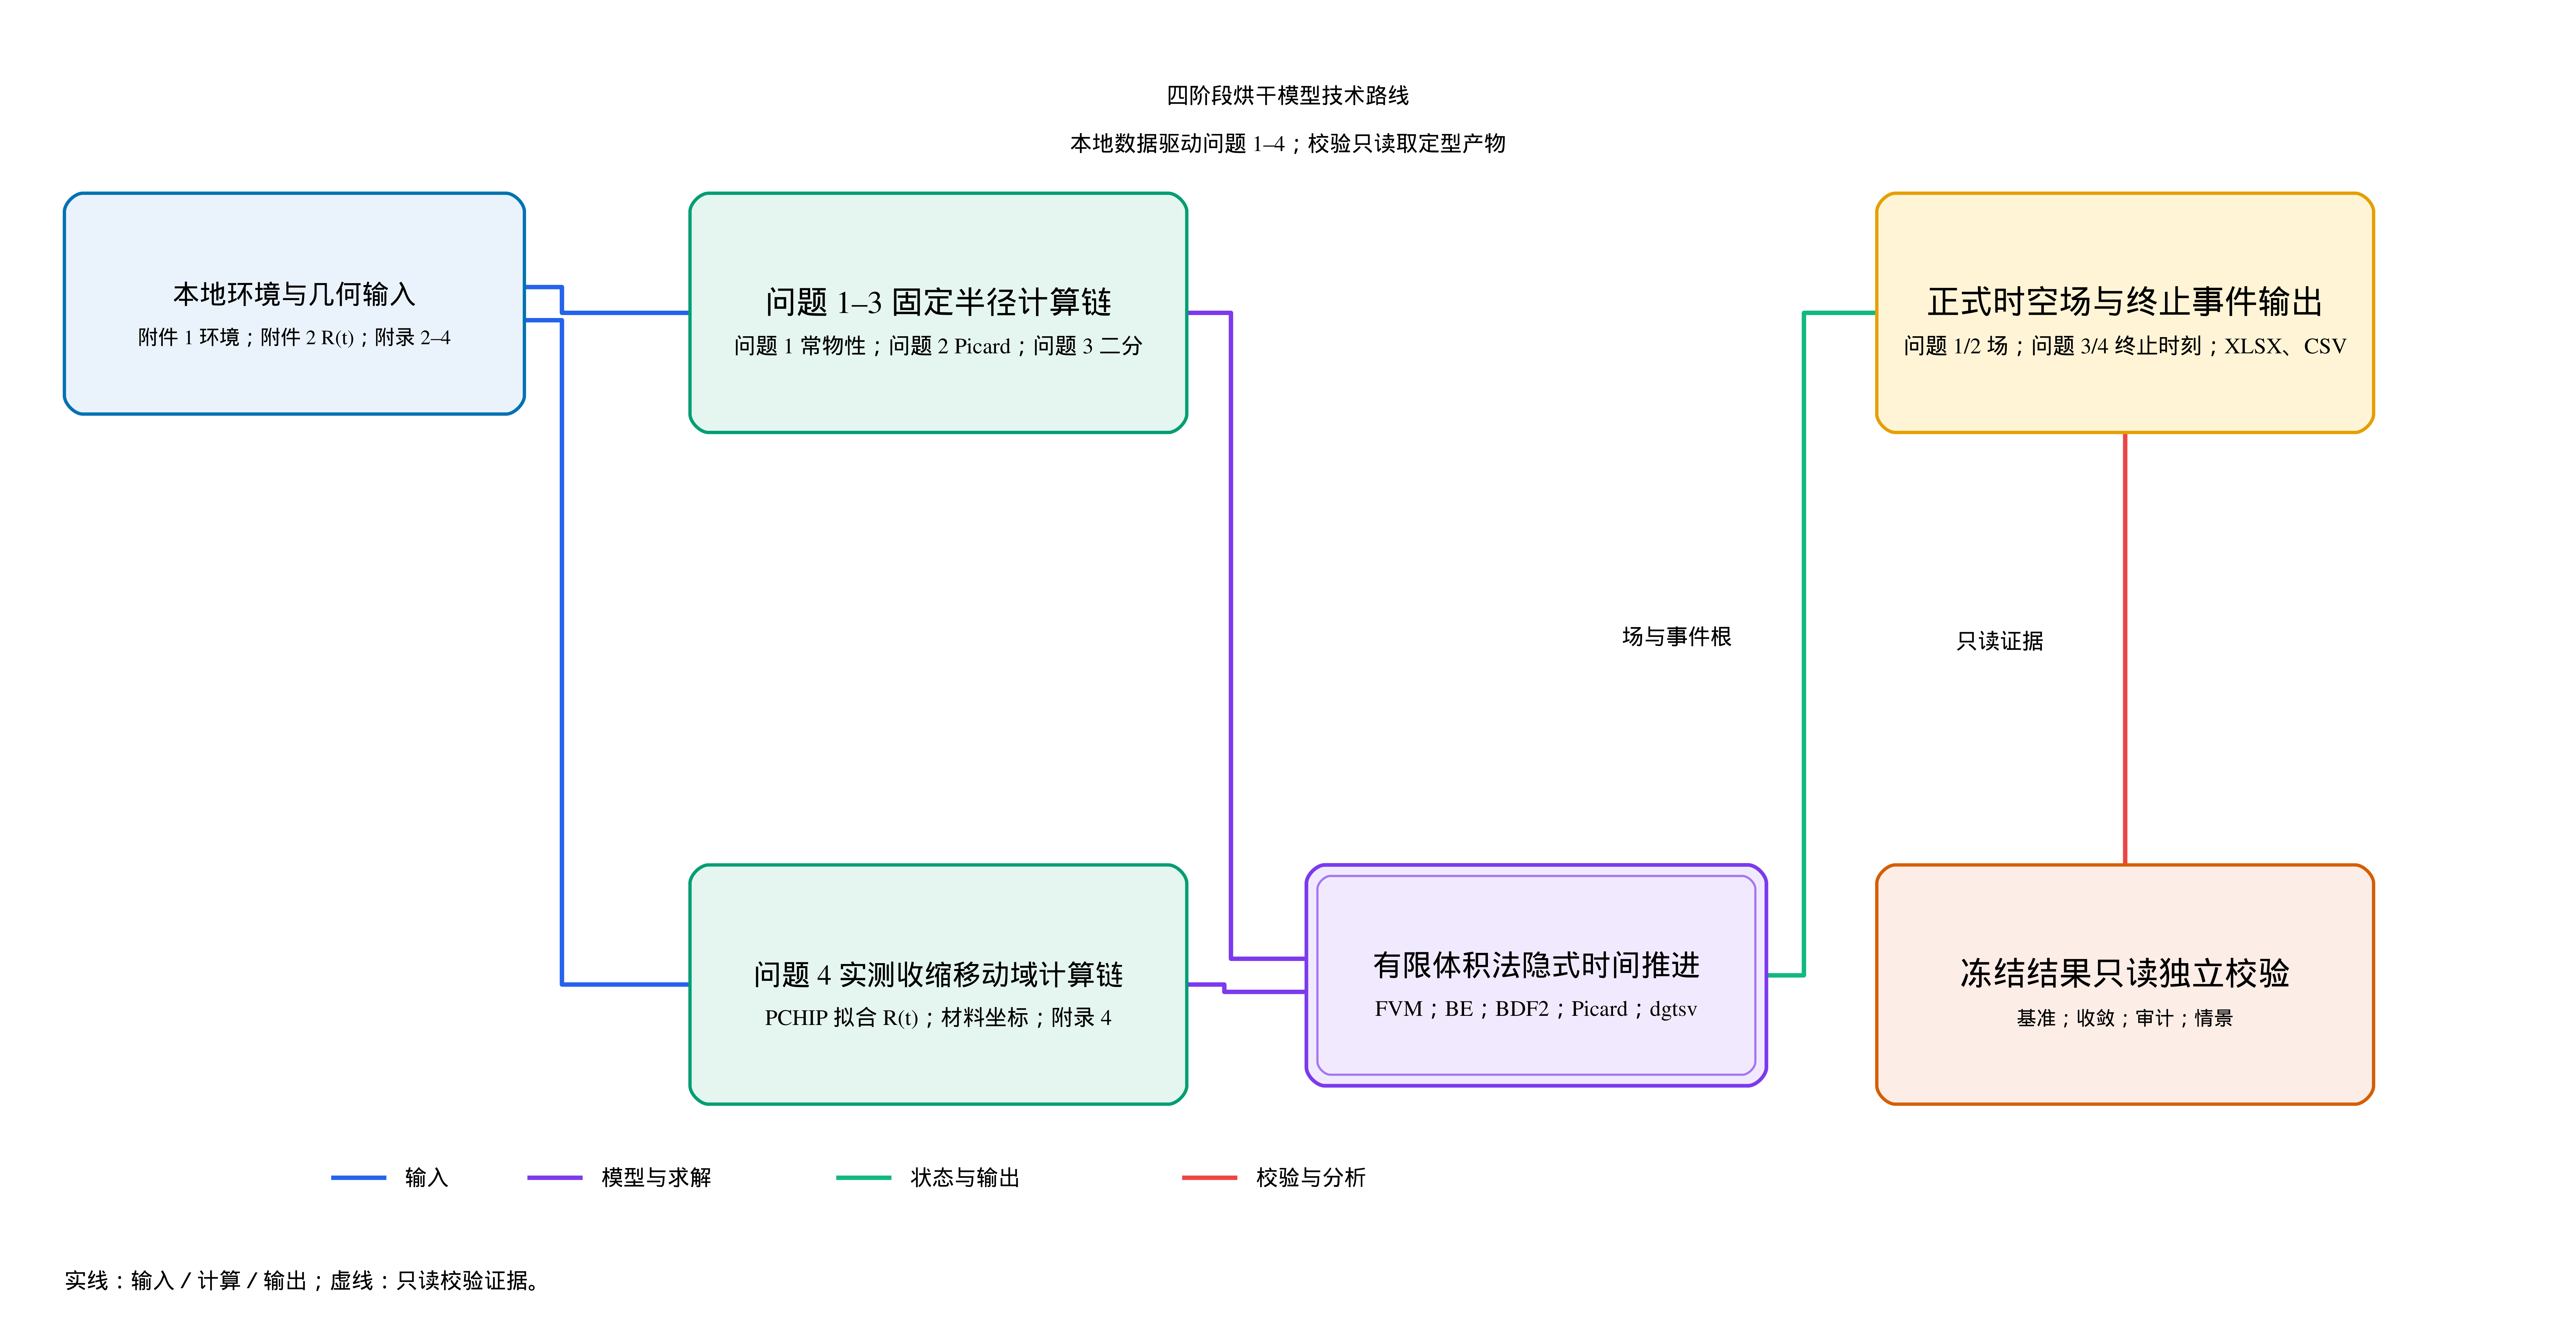
\includegraphics[width=0.96\textwidth]{figures/model_route}
  \caption{四阶段技术路线：本地输入驱动固定域与实测收缩域模型，正式结果经只读验证与情景分析检验}
  \label{fig:route}
\end{figure}

图中上半支为固定半径计算链（问题一至三），下半支为实测收缩移动域计算链
（问题四），两支共享同一套有限体积时间推进与事件定位模块，并由右侧的
校验模块只读复核。

\noindent\textbf{问题一（单向驱动的弱耦合抛物型方程）。}
【数学本质】时变 Robin 边界下圆柱坐标系的一维非稳态扩散初边值问题。
【状态与约束】状态量为 $T(r,t)$、$X(r,t)$，约束为径向均匀初值、中心
对称条件与表面 Robin 边界。
【求解难点与拟用算法】核心物理特征是表面强对流传质导致的边界层现象——
表层水分骤降而中心尚未响应，其空间梯度远陡于常规网格尺度，粗网格会把
局部梯度误写成整体脱水。拟采用单元中心有限体积法离散，并配合隐式时间
推进（Backward Euler 启动、变步长 BDF2）以保证陡梯度下的数值稳定性；
边界层分辨率由表面水分的空间与时间加密试验单独检验，而非仅比较终点数值。

\noindent\textbf{问题二（参数型双向强耦合非线性抛物型方程）。}
【数学本质】物性系数 $\rho,c_p,k$ 依赖 $X$、有效扩散系数依赖
$(X,\Theta)$ 的变系数抛物型方程组。
【状态与约束】状态量与问题一相同，但物性不再冻结，形成
$X\to\rho,c_p,k\to T$ 与 $(T,X)\to D_{\mathrm{eff}}\to X$ 的双向闭环。
【求解难点与拟用算法】直接显式推进受稳定性限制，故每个时间层以 Picard
迭代冻结并更新系数；界面导热与扩散系数取调和平均，表面 Robin 条件按
半单元扩散阻力与对流阻力串联离散，以在强非线性下保持迭代收敛。

\noindent\textbf{问题三（PDE 场解上的连续不等式首次穿越）。}
【数学本质】连续状态空间上的根定位事件问题，而非新的偏微分方程。
【状态与约束】在问题二的场解上定义事件函数
$g(t)=\max_{0\le r\le R_0}X(r,t)-0.15$；降速干燥阶段各点含水率单调衰减，
故 $X_{\max}(t)$ 连续且单调不增，$g(t)$ 亦连续且单调不增，其零点唯一。
【求解难点与拟用算法】真实终止时刻一般不与离散时间节点重合，若直接取
规则 $60\ \mathrm{s}$ 输出行将引入采样截断误差。利用 $g$ 的连续单调性，
先用相邻时间层的符号变化括住零点，再在区间内以二分法定位连续终止时刻，
从而把事件精度与输出采样间隔解耦。

\noindent\textbf{问题四（外部实测几何驱动的移动边界 PDE）。}
【数学本质】求解域 $r\in[0,R(t)]$ 随时间收缩的移动边界问题，几何由外部
实测给定，而非由水分场反演收缩本构。
【状态与约束】状态量仍为 $T,X$，但物理域随 $R(t)$ 收缩，且固定物理位置
一旦越出收缩域即不再外推。
【求解难点与拟用算法】若在物理坐标下随域重构网格，将引入插值误差与时变
网格管理成本。拟引入材料坐标 $\xi=r/R(t)\in[0,1]$ 将动域映射为固定域，
配合 PCHIP 保形插值抑制实测序列末端的伪振荡；该变换把几何收缩对传质
路径的贡献与附录物性差异分离开来。

\noindent\textbf{独立校验与工艺比较。}
主求解器的正式输出定型后，解析基准、空间与时间收敛、工作簿审计和通量
闭合分别检验方程、离散、交付与数值一致性；敏感性和平台温度扫描只消费
这些定型结果。其评价指标为 $t_{\mathrm{dry}}$ 与终点含水率均匀性；由于
当前模型不含品质降解和能耗机理，温度扫描仅给出考察区间内的条件性比较，
不宣称生产全局最优。

% ==================== 三、模型假设 ====================
\section{模型假设}

\begin{enumerate}
  \item \textbf{一维轴对称等效介质。}考虑到药材长度与半径之比为 $12.5$、端面总
  面积约为侧面积的 $8\%$，且热风周向条件近似均匀，假设药材为连续、
  均匀、各向同性的圆柱等效介质，初始温湿场在径向上均匀。由此以
  $T(r,t),X(r,t)$ 替代三维场，并给出式 \eqref{eq:energy}--
  \eqref{eq:moisture}、中心对称条件及式 \eqref{eq:ic} 的一维初边值问题。
  \item \textbf{表面对流闭合。}考虑到题目仅给出对流换热、传质系数且未
  提供辐射参数，假设外界只经表面对流与药材交换热量和有效水分势；附录
  3、4 未给新系数时沿用基准 $h_T,h_m$。由此将外界输入写为式
  \eqref{eq:bc-T}--\eqref{eq:bc-X} 的 Robin 边界，并在第八节对该缺省
  闭合进行灵敏度检验。
  \item \textbf{经验有效扩散而非相变守恒闭合。}考虑到现有数据不能由
  $h_m(X_s-\chi_a)$ 唯一恢复真实水蒸气质量通量或局部相变速率，假设水分
  迁移可由干基含水率的经验有效扩散表示，而不另设潜热源项。由此水分采用
  式 \eqref{eq:moisture} 的通量形式，能量方程保持式 \eqref{eq:energy}，
  不把数值通量闭合解释为设备尺度的完整质量或能量守恒。
  \item \textbf{长期环境平台延拓。}考虑到附件 1 只覆盖前 $4\ \mathrm{h}$，
  而问题 3、4 的终止事件跨越更长时间，假设其后烘房环境维持末端实测平台
  值。由此将 $T_a(t),\chi_a(t)$ 在 $t>14400\ \mathrm{s}$ 延拓为常数，并
  在第八节用环境扰动情景检验这一外推对终止时间的影响。
  \item \textbf{实测半径的单向相似收缩。}考虑到附件 2 给出的是半径观测
  而非由水分场反演的收缩本构，假设 $R(t)$ 外部给定，且同一材料点的
  $\xi=r/R(t)$ 保持不变。由此用 PCHIP 构造并钳制 $R(t)$，在
  $\xi\in[0,1]$ 上得到式 \eqref{eq:energy-xi}--\eqref{eq:bc-xi} 的移动域
  计算，且不让温湿场反向改写半径轨迹。
\end{enumerate}

% ==================== 四、符号说明 ====================
\section{符号说明}

附件 1 的原始环境水分数值记为 $C_a$；进入 Robin 边界的有效水分势记为
$\chi_a$，基准闭合取 $\chi_a=C_a$。下表中同一符号的大小写、下标及单位
在全文保持一致。

{\renewcommand{\arraystretch}{1.12}
\begin{longtable}{@{}p{0.13\textwidth}p{0.32\textwidth}p{0.18\textwidth}p{0.25\textwidth}@{}}
\toprule
符号 & 含义 & 单位 & 属性/备注 \\
\midrule
\endfirsthead
\toprule
符号 & 含义 & 单位 & 属性/备注（续） \\
\midrule
\endhead
\bottomrule
\endfoot
\bottomrule
\endlastfoot
$r$ & 径向物理坐标 & $\mathrm{m}$ & Q1--Q3 的求解坐标 \\
$t$ & 时间 & $\mathrm{s}$ & 自变量 \\
$i,n$ & 径向单元、时间层索引 & 无量纲 & 数值离散索引 \\
$T,X$ & 药材温度、干基含水率 & $^\circ\mathrm{C}$；$\mathrm{kg\,kg^{-1}}$ & 状态变量 \\
$\Theta$ & 绝对温度，$\Theta=T+273.15$ & $\mathrm{K}$ & 派生状态；Arrhenius 项输入 \\
$T_s,X_s$ & 药材表面温度、表面含水率 & $^\circ\mathrm{C}$；$\mathrm{kg\,kg^{-1}}$ & 由表面控制体重构 \\
$T_a,C_a$ & 烘房温度、附件原始水分数值 & $^\circ\mathrm{C}$；$\mathrm{kg\,kg^{-1}}$ & 已知时变输入 \\
$\chi_a$ & Robin 边界的有效外部水分势 & $\mathrm{kg\,kg^{-1}}$ & 闭合量；基准取 $\chi_a=C_a$ \\
$R_0,R(t)$ & 初始半径、实测收缩半径 & $\mathrm{m}$ & 已知几何；Q4 的 $R(t)$ 由 PCHIP 给定 \\
$\xi$ & 材料坐标，$\xi=r/R(t)$ & 无量纲 & Q4 计算坐标 \\
$\rho,c_p,k,D_{\mathrm{eff}}$ & 密度、比热、导热系数、有效扩散系数 & 见表 \ref{tab:props} & 题目附录经验物性 \\
$h_T,h_m$ & 对流换热、等效传质系数 & $\mathrm{W\,m^{-2}\,K^{-1}}$；$\mathrm{m\,s^{-1}}$ & 已知/缺省闭合参数 \\
$\Gamma$ & 界面传递系数（$k$ 或 $D_{\mathrm{eff}}$） & 随对象而定 & 边界等效阻力参数 \\
$\delta$ & 表面半单元厚度，$R/(2N)$ & $\mathrm{m}$ & 数值离散量 \\
$h_{\mathrm{eff}}$ & 串联阻力的等效传递系数 & 同 $h$ & 派生边界参数 \\
$\bar X,\sigma_X$ & 截面积加权平均值、终点标准差 & $\mathrm{kg\,kg^{-1}}$ & 派生评价指标 \\
$g(t)$ & 事件函数，$\max_rX(r,t)-0.15$ & $\mathrm{kg\,kg^{-1}}$ & 派生约束量；$g(t)\le0$ 时终止 \\
$t_{\mathrm{dry}}$ & 烘干终止时间 & $\mathrm{s}$ & 事件定位输出 \\
$N$ & 径向网格单元数 & 无量纲 & 数值参数 \\
$\lambda_n$ & 圆柱导热问题特征值 & 无量纲 & 解析基准参数 \\
$\mathrm{Bi}$ & Biot 数 & 无量纲 & 无量纲边界参数 \\
\end{longtable}
}
\addtocounter{table}{-1} % 符号说明不计入论文表编号

% ==================== 五、模型建立 ====================
\section{模型建立}

\subsection{控制方程与定解条件（固定半径工况）}

在固定半径条件下（对应问题 $1$--$3$），药材几何区域保持不变，求解域
为：$0<r<R_0$。烘干过程中，药材内部同时存在热传导与水分迁移过程，
温度场与含水率场通过温度、含水率相关的物性参数实现耦合。温度场采用
能量方程，水分场采用以干基含水率为状态变量的经验有效扩散方程；后者
不宣称为严格的水分质量守恒本构。扩散方程保留变系数通量形式
\cite{crank1975}。相应的轴对称非稳态控制方程为：

\begin{equation}
  \rho(X)\,c_p(X)\,\frac{\partial T}{\partial t}
  =\frac{1}{r}\frac{\partial}{\partial r}
  \left[r\,k(X)\frac{\partial T}{\partial r}\right],
  \label{eq:energy}
\end{equation}

水分场控制方程为：

\begin{equation}
  \frac{\partial X}{\partial t}
  =\frac{1}{r}\frac{\partial}{\partial r}
  \left[r\,D_{\mathrm{eff}}(X,\Theta)\frac{\partial X}{\partial r}\right].
  \label{eq:moisture}
\end{equation}

其中，密度 $\rho(X)$、比热容 $c_p(X)$、导热系数 $k(X)$ 以及有效扩散
系数 $D_{\mathrm{eff}}(X,\Theta)$ 均根据药材温度与含水率状态动态变化，
从而描述烘干过程中热物性与传质特性的非线性变化。

式 \eqref{eq:energy}--\eqref{eq:moisture} 是问题 2、3 的参数型双向耦合
骨架：$X$ 改变 $\rho,c_p,k$ 并影响温度场，而 $(T,X)$ 共同决定
$D_{\mathrm{eff}}$。问题 1 则按附录 2 取常热物性，且 $D_1$ 仅依赖
$X$；故其温度场与水分场是受同一时变边界驱动的并行场，而非内部双向
耦合。该区别决定了问题 1 的专项边界层收敛验证和问题 2、3 的 Picard
非线性迭代不能混为一谈。

\subsubsection*{（1）初始条件}

按假设 1，将题设初始温湿状态作为径向均匀场，因此有：

\begin{equation}
  T(r,0)=28\ ^\circ\mathrm{C},\qquad
  X(r,0)=2.55\ \mathrm{kg\,kg^{-1}}.
  \label{eq:ic}
\end{equation}

\subsubsection*{（2）中心对称边界条件}

由于圆柱中心处不存在径向热流和水分通量，根据轴对称条件，有：

\begin{equation}
  \left.\frac{\partial T}{\partial r}\right|_{r=0}=0,\qquad
  \left.\frac{\partial X}{\partial r}\right|_{r=0}=0,
  \label{eq:bc-center}
\end{equation}

\subsubsection*{（3）表面对流边界条件}

药材表面 $r=R_0$ 与外部热风环境之间通过对流方式进行能量和质量交换，
因此采用 Robin 边界条件进行描述。对于热传递过程：

\begin{equation}
  k(X_s)\left.\frac{\partial T}{\partial r}\right|_{r=R_0}
  =h_T\,[T_a(t)-T_s(t)],
  \label{eq:bc-T}
\end{equation}

对于水分传递过程：

\begin{equation}
  -D_{\mathrm{eff}}(X_s,\Theta_s)
  \left.\frac{\partial X}{\partial r}\right|_{r=R_0}
  =h_m\,[X_s(t)-\chi_a(t)].
  \label{eq:bc-X}
\end{equation}

其中，$T_s(t)$ 和 $X_s(t)$ 分别表示药材表面温度与表面含水率，
$T_a(t)$ 和 $\chi_a(t)$ 分别表示外部烘房温度与进入边界的有效水分势；
基准闭合下 $\chi_a(t)=C_a(t)$。

\subsection{物性模型与环境输入}

各工况所需物性参数均采用题目附录给出的经验关联公式，具体形式汇总于表
\ref{tab:props}。计算过程中温度统一采用摄氏温度表示，仅在涉及
Arrhenius 指数项时转换为绝对温度：$\Theta=T+273.15\ \mathrm{K}$。
其中，含水率变量 $X$ 始终采用干基含水率表示。

\begin{table}[htbp]
  \centering
  \setcounter{table}{6} % 表 1--6 留给题目要求的六张表
  \caption{各工况物性经验公式（题目附录 2--4）}
  \label{tab:props}
  \resizebox{\textwidth}{!}{%
  \begin{tabular}{lllll}
  \toprule
  工况 & $\rho\ /\ \mathrm{kg\,m^{-3}}$ & $c_p\ /\ \mathrm{J\,kg^{-1}\,K^{-1}}$ &
  $k\ /\ \mathrm{W\,m^{-1}\,K^{-1}}$ & $D_{\mathrm{eff}}\ /\ \mathrm{m^2\,s^{-1}}$ \\
  \midrule
  附录 2（问题 1） & $820$ & $2600$ &
  $0.36$ & $7\times10^{-9}\,\mathrm{e}^{-0.89/X}$ \\
  附录 3（问题 2、3） & $650+128X$ & $1450+\dfrac{2736X}{X+1}$ &
  $0.21+\dfrac{0.38X}{X+1}$ &
  $2.4\times10^{-3}\,\mathrm{e}^{-0.45/X}\,\mathrm{e}^{-3850/\Theta}$ \\
  附录 4（问题 4） & $760+90X$ & $1850+\dfrac{2150X}{X+1}$ &
  $0.12+\dfrac{0.20X}{X+1}$ &
  $4.2\times10^{-4}\,\mathrm{e}^{-0.30/X}\,\mathrm{e}^{-3850/\Theta}$ \\
  \bottomrule
  \end{tabular}%
  }
\end{table}

其中，问题 1 采用附录 2 中的常物性参数，用于描述预热阶段的热湿
传递过程；问题 2 和问题 3 采用附录 3 中的变物性模型，使密度、比热容、
导热系数以及有效扩散系数随温度和含水率变化；问题 4 进一步采用附录 4
中的收缩条件物性模型，以反映药材失水收缩过程中材料性质的动态变化。

边界条件中的换热系数和传质系数分别取
$h_T=25\ \mathrm{W\,m^{-2}\,K^{-1}}$，
$h_m=8\times10^{-7}\ \mathrm{m\,s^{-1}}$。烘房环境输入数据由附件 1
提供。由于附录 3、4 未提供新的表面对流系数，问题 $2$--$4$ 的基准情景
沿用该取值，并在第八节通过敏感性分析评价这一缺省闭合假设。其中，观测
区间 $0\le t\le14400\ \mathrm{s}$ 内采用时间间隔为
$60\ \mathrm{s}$ 的实测温度与环境水分数据，并通过分段线性插值得到任意
时刻的环境状态。当 $t>14400\ \mathrm{s}$ 时，认为烘房进入恒温干燥
阶段，保持末端实测值不变，即
$T_a=50.165\ ^\circ\mathrm{C}$、$C_a=\chi_a=0.04986\ \mathrm{kg\,kg^{-1}}$，
如图 \ref{fig:env} 所示。

\begin{figure}[htbp]
  \centering
  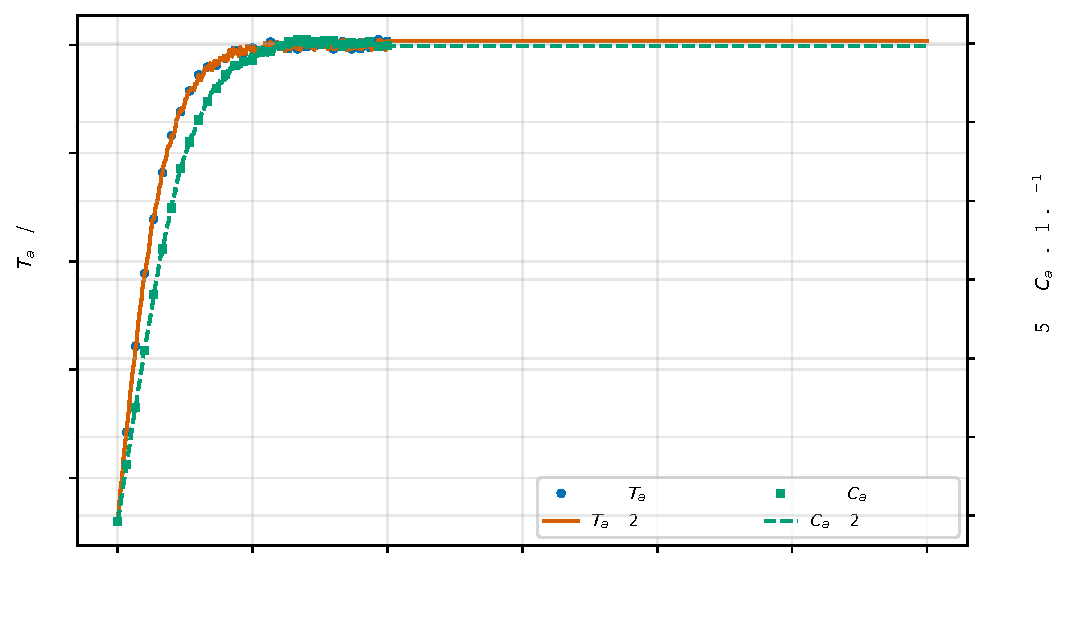
\includegraphics[width=0.88\textwidth]{figures/input_environment}
  \caption{烘房环境输入：实测温度（左轴）与水分势（右轴）的分段线性插值
  及 $4\ \mathrm{h}$ 后的平台延拓}
  \label{fig:env}
\end{figure}

\subsection{收缩移动域模型（问题 4）}

问题 4 进一步考虑药材失水过程中的几何收缩效应，此时药材半径 $R(t)$
随时间变化，导致计算区域成为动态移动边界。为避免直接在物理坐标下处理
随时间变化的计算域，引入材料坐标：$\xi=r/R(t)$，$0\le\xi\le1$。将随
时间变化的物理区域映射至固定区域 $[0,1]$，从而将移动边界问题转化为
固定计算域上的变系数偏微分方程问题。

具体地，径向相似收缩使固定 $\xi$ 对应同一材料点，且
\[
  r=R(t)\xi,\qquad \frac{\partial}{\partial r}
  =\frac{1}{R(t)}\frac{\partial}{\partial\xi}.
\]
因此材料导数可直接写为固定 $\xi$ 下的时间导数；径向扩散算子中的两个
空间导数各带来一个 $1/R(t)$。代入固定域通量形式即得收缩条件下的温度场
控制方程：

\begin{equation}
  \rho_4(X)\,c_{p,4}(X)\,\frac{\partial T}{\partial t}
  =\frac{1}{R(t)^2\,\xi}\frac{\partial}{\partial\xi}
  \left[\xi\,k_4(X)\frac{\partial T}{\partial\xi}\right],
  \label{eq:energy-xi}
\end{equation}

水分场控制方程为：

\begin{equation}
  \frac{\partial X}{\partial t}
  =\frac{1}{R(t)^2\,\xi}\frac{\partial}{\partial\xi}
  \left[\xi\,D_4(X,\Theta)\frac{\partial X}{\partial\xi}\right].
  \label{eq:moisture-xi}
\end{equation}

其中，$\rho_4(X)$、$c_{p,4}(X)$、$k_4(X)$ 和 $D_4(X,\Theta)$ 分别表示
考虑收缩条件下药材的密度、比热容、导热系数以及有效水分扩散系数。

在固定计算域边界 $\xi=1$ 处，仍采用 Robin 边界条件描述药材与外部
环境之间的热量和水分交换：

\begin{equation}
  \frac{k_4(X_s)}{R(t)}
  \left.\frac{\partial T}{\partial\xi}\right|_{\xi=1}
  =h_T\,[T_a(t)-T_s(t)],\qquad
  -\frac{D_4(X_s,\Theta_s)}{R(t)}
  \left.\frac{\partial X}{\partial\xi}\right|_{\xi=1}
  =h_m\,[X_s(t)-\chi_a(t)].
  \label{eq:bc-xi}
\end{equation}

半径变化函数 $R(t)$ 根据附件 2 提供的实测半径数据构造。具体而言，采用
PCHIP 保形插值方法对 $0$--$72\ \mathrm{h}$ 内、时间间隔为
$1800\ \mathrm{s}$ 的实验数据进行拟合。相比传统三次样条插值，PCHIP
方法能够保持数据单调性，避免末端平台阶段附近出现非物理振荡。根据实测
结果，当 $t\ge241200\ \mathrm{s}$ 后，连续 $11$ 个测量点均保持半径约为
$1.198\ \mathrm{cm}$，因此将后续半径固定为平台值：
$R=0.01198\ \mathrm{m}$。同时，将实验半径数据由厘米转换为米，并在程序
输入层校验初始条件：$R(0)=0.02\ \mathrm{m}$，以保证收缩模型与固定半径
模型在初始时刻保持连续一致。

\subsection{数值求解方案}

四个问题均采用统一的有限体积数值求解框架，仅根据物性模型、几何条件
以及输出需求进行相应调整。其中，问题 $1$--$3$ 采用固定半径计算域，
问题 4 通过材料坐标变换处理收缩导致的移动边界问题。

\subsubsection*{（1）空间离散}

采用\textbf{单元中心有限体积法（cell-centered finite volume method）}
进行空间离散：问题 $1$--$3$ 在物理半径域 $r\in[0,R_0]$ 上离散，问题
4 在材料坐标域 $\xi\in[0,1]$ 上离散。对于径向网格划分，第 $i$ 个控制
体每单位轴向长度的截面积与对应环形区域一致；这一有限体积处理与数值传热中
的守恒离散思想一致\cite{tao2001,patankar1980}。即：

\begin{equation*}
  V_i=\pi R^2\frac{(2i-1)}{N^2}.
\end{equation*}

其中，问题 $1$--$3$ 中取固定半径 $R\equiv R_0$，问题 4 中取时变半径
$R\equiv R(t)$。该离散方式能够保证控制体尺度与圆柱轴对称几何结构相
匹配，从而保持径向传热和经验有效扩散方程的离散通量一致性。

对统一的径向通量形式在第 $i$ 个控制体上积分，内外界面通量相减；在等距
网格下，界面面积与中心距相除后化为 $2\pi i$ 和 $2\pi(i-1)$。故温度场
的半离散式为：

\begin{equation}
  \rho c_p\,V_i\,\frac{\mathrm dT_i}{\mathrm dt}
  =2\pi i\,k_{i+1/2}\left(T_{i+1}-T_i\right)
  -2\pi(i-1)\,k_{i-1/2}\left(T_i-T_{i-1}\right),
  \label{eq:fvm}
\end{equation}

其中，$V_i$ 是每单位轴向长度的控制体截面积，$k_{i\pm1/2}$ 取相邻单元
的调和平均；水分方程沿用同一界面通量结构，只将左端热容系数
$\rho c_p$ 改为 $1$，并把 $k$ 替换为 $D_{\mathrm{eff}}$。

\subsubsection*{（2）中心点与界面处理}

在圆柱中心处，由于控制体面积趋于零，轴对称条件自然满足。对于水分控制
方程，其时间项系数取为 $1$，即不包含 $\rho c_p$ 项。

对于内部网格界面，采用相邻控制体物性参数的调和平均方式计算界面扩散
系数，以保证扩散通量在单元界面处连续，并避免由于物性突变导致的数值
振荡。同时，对中心边界进行特殊处理，避免因径向坐标趋近于零而产生
$0/0$ 数值问题。

\subsubsection*{（3）边界通量处理}

对于表面控制体，Robin 边界条件通过等效扩散阻力形式进行离散处理。将
半单元内部扩散阻力与表面对流阻力串联，得到等效传递系数：

\begin{equation}
  h_{\mathrm{eff}}=\frac{h\,\Gamma}{\Gamma+h\,\delta},\qquad
  \Gamma\in\{k,D_{\mathrm{eff}}\},
  \label{eq:heff}
\end{equation}

其中，$\delta=R/(2N)$ 表示表面控制体厚度。该处理方式可使边界通量与
内部扩散通量保持一致，并维持离散矩阵的三对角结构，避免显式二阶外推
可能导致的负权重问题。同时，表面温度 $T_s$ 与表面含水率 $X_s$ 通过
上述串联阻力关系由最外层控制体反算获得。

\subsubsection*{（4）时间离散}

时间推进采用隐式格式。首先使用 Backward Euler 方法完成初始两步计算，
随后采用变步长 BDF2 格式提高时间离散精度\cite{gear1971}。令
$\theta=\Delta t/\Delta t_{-1}$，则 BDF2 离散格式表示为：

\begin{equation}
  u_{n+1}=\frac{(1+\theta)^2u_n-\theta^2u_{n-1}}{2\theta+1}
  +\frac{\theta(1+\theta)\,\Delta t_{-1}}{2\theta+1}\,f(u_{n+1}),
  \label{eq:bdf2}
\end{equation}

该格式具有无条件稳定性，并保持二阶时间精度。时间步长根据工况与计算阶段
动态调整：

\begin{itemize}
  \item 问题 1 取 $N=2561$、$\Delta t_{\max}=0.03125\ \mathrm{s}$，
  用于分辨 $t=1\ \mathrm{s}$ 的强表面边界层；
  \item 问题 2--4 基准计算取 $N=321$、$\Delta t_{\max}=60\ \mathrm{s}$，
  低含水率末期将步长收紧至不超过 $20\ \mathrm{s}$；
  \item 时间推进强制落在附件 1 的 $60\ \mathrm{s}$ 边界数据节点；正式
  工作簿和论文表的保存间隔则按各问题的输出契约另行抽样。
\end{itemize}

\subsubsection*{（5）非线性迭代求解}

由于物性参数依赖温度和含水率，离散后的控制方程具有明显的非线性特征。
每个时间步内采用 Picard 迭代，将物性参数冻结于上一迭代步，并不断更新
温度场与含水率场。迭代收敛条件分别设置为：
$\max|\Delta T|<10^{-7}\ ^\circ\mathrm{C}$，
$\max|\Delta X|<10^{-8}\ \mathrm{kg\,kg^{-1}}$。同时，在低含水率末期
引入停滞检测机制（松弛因子取 $0.5$），以保证固定点迭代过程稳定收敛。
线性化后的三对角方程组采用 LAPACK 中的 \texttt{dgtsv} 函数直接求解；
具体实现调用 SciPy 数值计算库\cite{virtanen2020}。

\subsubsection*{（6）事件定位}

问题 3 和问题 4 分别以固定域和材料域上的全域最大含水率定义连续事件：

\begin{equation}
  \begin{aligned}
    g_3(t)&=\max_{0\le r\le R_0}X(r,t)-0.15,\\
    g_4(t)&=\max_{0\le \xi\le1}X(\xi,t)-0.15.
  \end{aligned}
  \label{eq:event}
\end{equation}

真实终止时刻通常不与离散时间节点重合。当相应 $g_q(t)$ 在区间
$[t_k,t_{k+1}]$ 内发生符号变化时，保留跨越前时刻的完整积分器状态（包括
BDF2 历史信息和自适应步长状态）作为初值，在该区间内采用二分法求解
$g_q(t)=0$，得到
精确终止时刻 $t_{\mathrm{dry}}$。事件定位容差设置为 $0.01\ \mathrm{s}$，
并返回该时刻对应的完整温度场和含水率场。

\subsubsection*{（7）实现步骤与可复现配置}

计算使用 Python 3.11、NumPy、SciPy、pandas、openpyxl 与 Matplotlib 实现；
非线性时间层中的三对角线性系统由 SciPy 对 LAPACK \texttt{dgtsv} 的接口
求解。具体流程如下：

\begin{enumerate}[label=\textbf{Step \arabic*:}, leftmargin=2.6cm]
  \item 读取附件 1 的环境序列并作分段线性插值；问题 4 另读取附件 2，
  将厘米半径换为米后以 PCHIP 插值，并在 $241200\ \mathrm{s}$ 后钳制
  为 $0.01198\ \mathrm{m}$。
  \item 按问题选择附录物性、固定半径或材料坐标网格；在每个 Picard
  迭代内更新单元物性、调和平均界面系数及半单元 Robin 阻力。
  \item 以 Backward Euler 启动并切换至变步长 BDF2；每步以
  \[
    \|T^{(m+1)}-T^{(m)}\|_\infty<10^{-7},\qquad
    \|X^{(m+1)}-X^{(m)}\|_\infty<10^{-8}
  \]
  作为 Picard 收敛条件。
  \item 按题目契约采样温湿场；问题 3、4 监测 $g_q$ 的符号变化并二分
  定位事件，同时单独保存连续事件行而不以规则输出行替代。
  \item 主求解器输出定型后，运行解析基准、空间/时间收敛、通量闭合与工作簿
  审计；灵敏度和平台温度情景仅读取这些正式产物。
\end{enumerate}

% ==================== 六、模型求解与结果分析 ====================
\section{模型求解与结果分析}

\subsection{问题一：预热阶段}

预热阶段的特征扩散时间尺度可由热扩散估算：
$t_h\approx R_0^2/\alpha_1$，其中
$\alpha_1=k/(\rho c_p)=1.69\times10^{-7}\ \mathrm{m^2\,s^{-1}}$，
计算得到 $t_h\approx2369\ \mathrm{s}$。该时间尺度与题目要求考察的
$1800\ \mathrm{s}$ 时间范围处于同一数量级，说明预热阶段内部温度场
尚未达到稳定状态。因此，不能采用稳态近似，而需通过耦合热湿传递模型
求解完整的瞬态过程。

由于初始阶段表面水分迅速迁移，$t=1\ \mathrm{s}$ 时表面附近形成的水分
梯度层厚度约为 $\sqrt{D_1(X_0)t}\approx7.0\times10^{-5}\ \mathrm{m}=0.007\ \mathrm{cm}$（取 $D_1(X_0)=4.94\times10^{-9}\ \mathrm{m^2\,s^{-1}}$、$t=1\ \mathrm{s}$），常规空间网格难以充分解析该局部
变化。为保证计算结果达到四位小数精度，进行了网格与时间步长收敛性
验证，最终选取：$N=2561$，$\Delta t=0.03125\ \mathrm{s}$。在该计算
设置下，初始时刻表面含水率变化能够稳定收敛（见第 7.4 节）。

模型计算得到的问题一结果汇总于表 \ref{tab:t1} 和表 \ref{tab:t2}，
其中给出了 $100$、$300$、$600$、$900$、$1200$、$1500$ 以及
$1800\ \mathrm{s}$ 时刻，不同径向位置处的温度和含水率分布。
完整时间步长为 $1\ \mathrm{s}$、空间步长为 $0.1\ \mathrm{cm}$ 的计算
结果存储于 \texttt{result1.xlsx}。

\setcounter{table}{0} % 表 1--6 与题目表号一一对应

\input{tables/t1.tex}
\input{tables/t2.tex}

\begin{figure}[htbp]
  \centering
  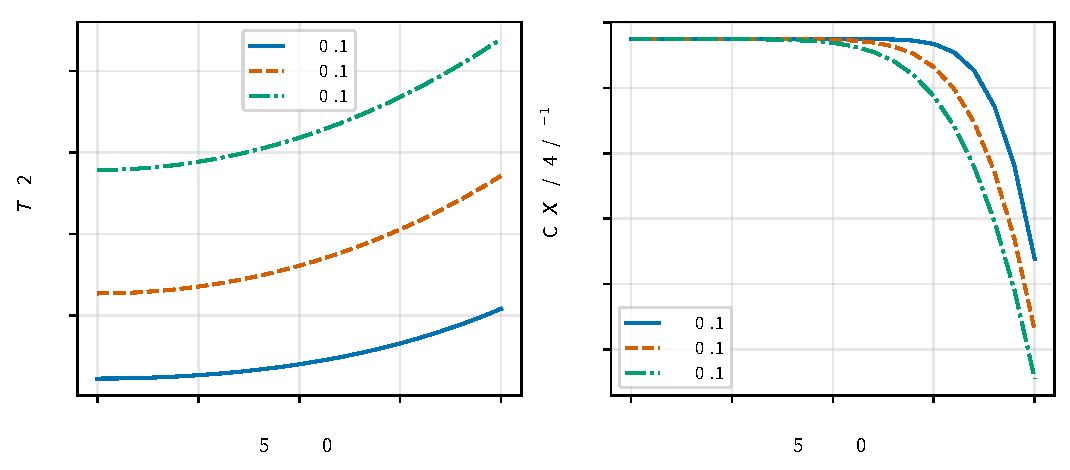
\includegraphics[width=0.82\textwidth]{figures/q1_profiles}
  \caption{预热阶段温度（左）与干基含水率（右）径向剖面}
  \label{fig:q1}
\end{figure}

由图 \ref{fig:q1} 可知，烘干过程中热量主要由药材表面向中心区域逐渐
传递。经过 $1800\ \mathrm{s}$ 后，药材表面温度升高至
$36.79\ ^\circ\mathrm{C}$，中心温度达到 $33.58\ ^\circ\mathrm{C}$，
径向温差约为 $3.2\ ^\circ\mathrm{C}$，表明温度场已逐渐趋于均匀，但仍
具有明显的非稳态传热特征。

相比之下，水分迁移具有更强的滞后性，主要集中发生于表层区域。
$1800\ \mathrm{s}$ 时，表面含水率由初始值
$2.5500\ \mathrm{kg\,kg^{-1}}$ 降低至
$1.5102\ \mathrm{kg\,kg^{-1}}$，而中心区域含水率仍保持为
$2.5500\ \mathrm{kg\,kg^{-1}}$，尚未出现明显的脱水现象。

造成热量扩散快于水分迁移的主要原因在于两者的扩散尺度存在差异。计算中
有效水分扩散系数为 $D_{\mathrm{eff}}\sim4\times10^{-9}\ \mathrm{m^2\,s^{-1}}$（$D_1(X_0)=4.94\times10^{-9}\ \mathrm{m^2\,s^{-1}}$，表面含水率降至 $1.51$ 时约为 $3.9\times10^{-9}\ \mathrm{m^2\,s^{-1}}$），
明显低于热扩散系数
$\alpha_1=1.69\times10^{-7}\ \mathrm{m^2\,s^{-1}}$，二者相差约 $35$--$44$ 倍。因此，温度场能够较快趋于均匀，而水分场由于迁移阻力较大，
表现出明显的表层优先脱水和内部水分滞后特征。

\subsection{问题二：完整烘干过程（前 3 小时）}

问题二和问题三均采用附录 3 给出的变物性经验模型（见表
\ref{tab:props}），考虑药材温度与含水率变化对密度、比热容、导热系数
以及有效扩散系数的影响，并对完整干燥过程进行数值模拟，直至达到终止
条件。

首先分析干燥初始阶段（前 $3$ 小时）的温度场与含水率场演化规律。图
\ref{fig:q2} 展示了该阶段不同时间下药材内部温度与含水率的分布情况，表
\ref{tab:t3} 和表 \ref{tab:t4} 分别给出了题目要求的采样时刻及不同径向
位置处的计算结果。

\begin{figure}[htbp]
  \centering
  \begin{minipage}{0.48\textwidth}
    \centering
    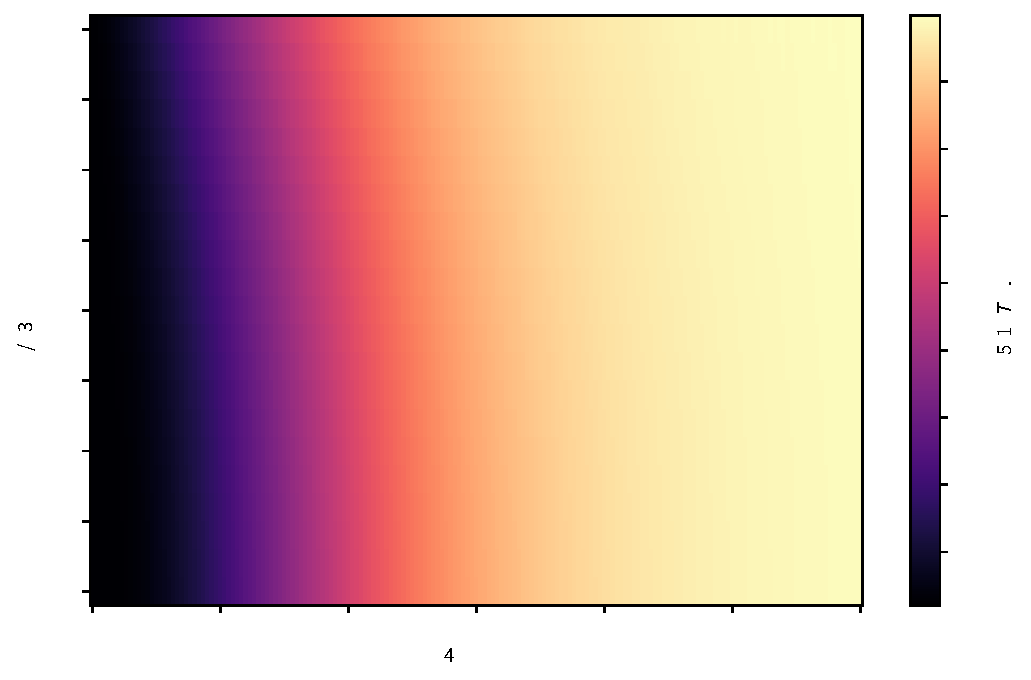
\includegraphics[width=\textwidth]{figures/q2_temperature_heatmap}
  \end{minipage}
  \hfill
  \begin{minipage}{0.48\textwidth}
    \centering
    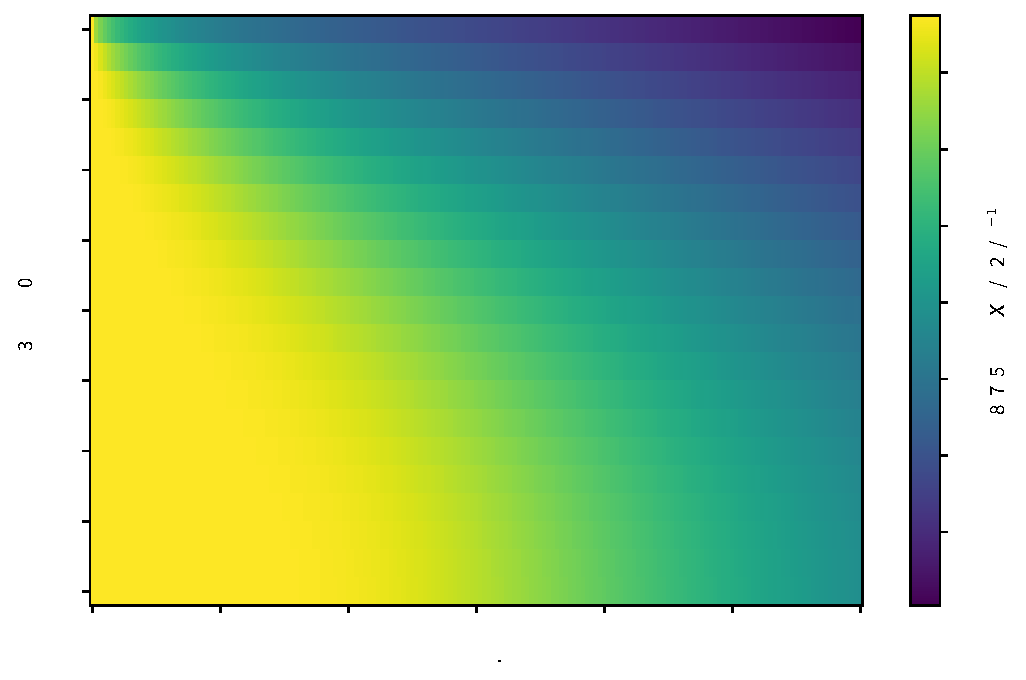
\includegraphics[width=\textwidth]{figures/q2_moisture_heatmap}
  \end{minipage}
  \caption{固定半径工况前三小时温度场（左）与含水率场（右）}
  \label{fig:q2}
\end{figure}

% 自动生成：python paper/build_tables.py（勿手工编辑）
\begin{table}[htbp]
\centering
\caption{烘干前 3 小时不同时刻的温度分布（单位：℃）}
\label{tab:t3}
\begin{tabular}{lccccc}
\toprule
时间/h & 0 cm & 0.5 cm & 1 cm & 1.5 cm & 2 cm \\
\midrule
0 & 28.0000 & 28.0000 & 28.0000 & 28.0000 & 28.0000 \\
0.5 & 32.1893 & 32.3821 & 32.9659 & 33.9608 & 35.4130 \\
1 & 40.3816 & 40.5536 & 41.0605 & 41.8782 & 42.9976 \\
1.5 & 45.8468 & 45.9348 & 46.1929 & 46.6051 & 47.1400 \\
2 & 48.4502 & 48.4881 & 48.5984 & 48.7735 & 49.0033 \\
2.5 & 49.4670 & 49.4792 & 49.5136 & 49.5653 & 49.6609 \\
3 & 49.8495 & 49.8553 & 49.8746 & 49.9101 & 49.9664 \\
\bottomrule
\end{tabular}
\end{table}

\input{tables/t4.tex}

前 $3$ 小时内，药材经历由预热阶段向恒温干燥阶段的过渡过程。温度场
响应较快，约在 $1$--$1.5\ \mathrm{h}$ 后，药材内部温度基本接近烘房
温度；$3\ \mathrm{h}$ 时径向温差仅约 $0.12\ ^\circ\mathrm{C}$（中心温度
$49.85\ ^\circ\mathrm{C}$，表面温度 $49.97\ ^\circ\mathrm{C}$），
表明温度分布已趋于均匀。

相比之下，含水率场的变化具有明显的滞后性，仍保持由表面向内部逐渐
递增的径向梯度。$3\ \mathrm{h}$ 时，表面含水率由初始值
$2.5500\ \mathrm{kg\,kg^{-1}}$ 降低至
$1.0081\ \mathrm{kg\,kg^{-1}}$，而中心区域含水率仍为
$1.7662\ \mathrm{kg\,kg^{-1}}$，表明内部水分尚未完全迁移至表面。由此
可见，在该阶段热量传递已基本完成，而水分扩散过程仍占主导作用，内部
水分迁移成为限制干燥速率的主要因素。

\subsection{问题三：烘干终止时间}

问题三以干基含水率达到终止条件作为干燥过程的结束判据，重点分析完整干燥
过程中药材内部含水率的时空演化规律。图 \ref{fig:q3-field} 展示了不同
时间下药材内部含水率的径向分布变化，图 \ref{fig:q3-summary} 进一步
给出了中心含水率、截面积加权平均含水率以及表面含水率随时间的变化
趋势。通过上述指标，可以综合评价干燥过程中表层与内部的水分迁移差异，
并确定满足：$\max_r X(r,t)\le0.15\ \mathrm{kg\,kg^{-1}}$ 条件下的精确
烘干终止时间。

\begin{figure}[htbp]
  \centering
  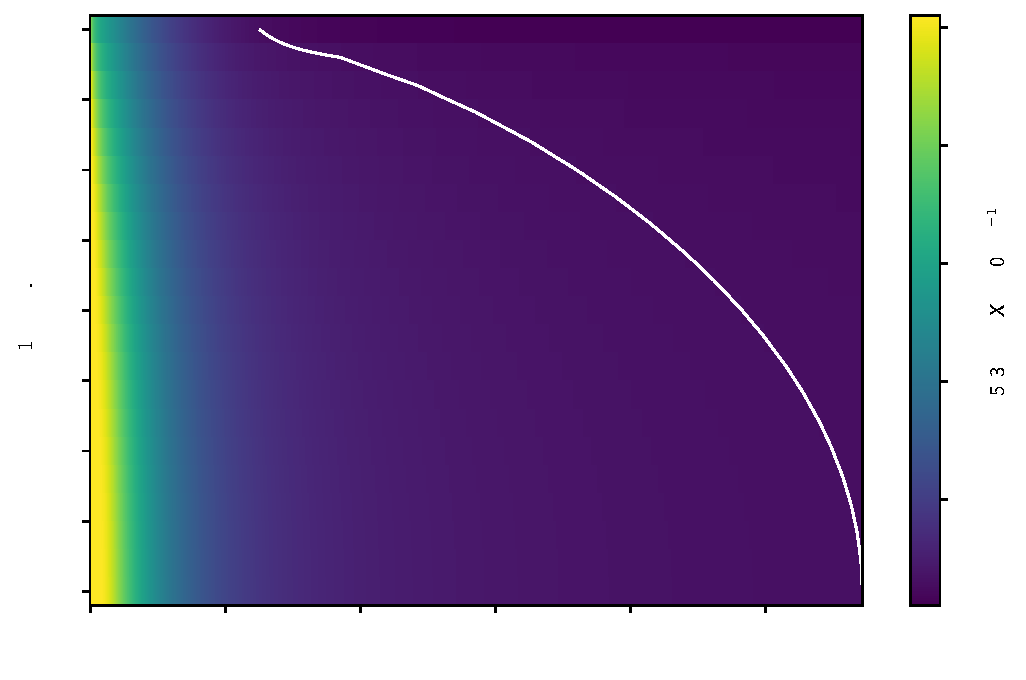
\includegraphics[width=0.82\textwidth]{figures/q3_moisture_heatmap}
  \caption{固定半径工况完整含水率时空分布（白色等值线为 $0.15$ 判据）}
  \label{fig:q3-field}
\end{figure}

\begin{figure}[htbp]
  \centering
  \begin{minipage}{0.48\textwidth}
    \centering
    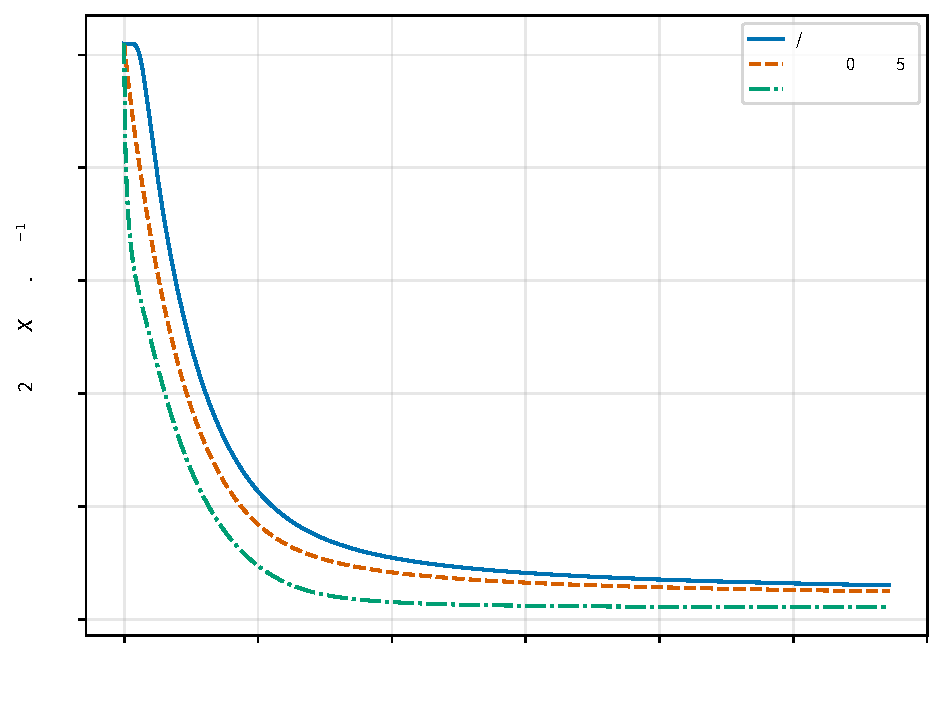
\includegraphics[width=\textwidth]{figures/q3_moisture_summary}
  \end{minipage}
  \hfill
  \begin{minipage}{0.48\textwidth}
    \centering
    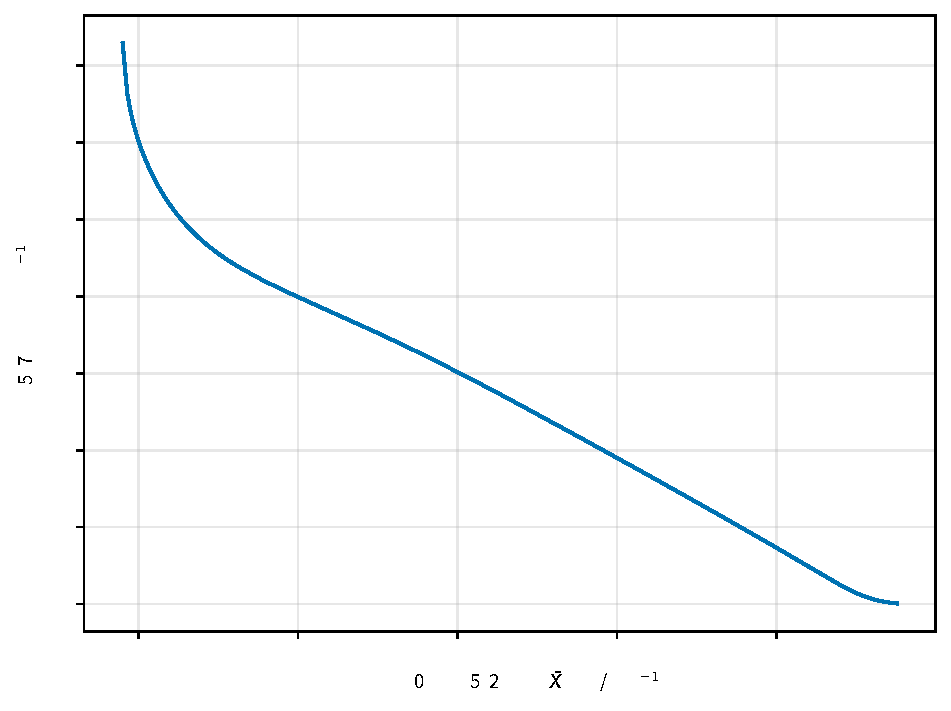
\includegraphics[width=\textwidth]{figures/q3_drying_rate}
  \end{minipage}
  \caption{中心、截面积加权平均与表面含水率（左）；平均干燥速率随平均
  含水率的变化（右）}
  \label{fig:q3-summary}
\end{figure}

\begin{figure}[htbp]
  \centering
  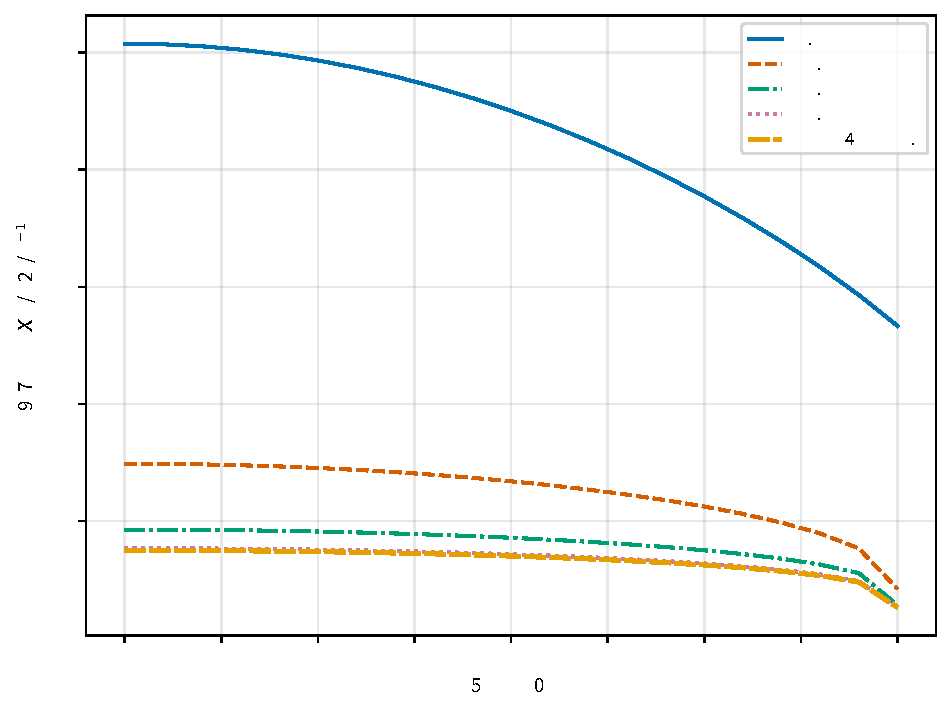
\includegraphics[width=0.82\textwidth]{figures/q3_profiles}
  \caption{固定半径工况不同时刻的含水率径向剖面}
  \label{fig:q3-profiles}
\end{figure}

\input{tables/t5.tex}

由图 \ref{fig:q3-summary} 可知，干燥过程中表面含水率下降最快，并在
初始阶段迅速接近环境平衡状态；相比之下，中心区域含水率下降最为缓慢，
最终干燥终止事件主要由内部含水率水平决定。随着平均含水率持续降低，
整个干燥过程始终处于降速干燥阶段，表明内部水分扩散阻力逐渐占据主导
作用。

基于前文构造的连续事件函数（式 \ref{eq:event}），通过事件穿越定位得到
满足终止条件：$\max_r X(r,t)\le0.15$ 的精确时刻为：

\begin{equation}
  t_{\mathrm{dry}}^{(3)}=205885.5\ \mathrm{s}=57.1904\ \mathrm{h},
  \label{eq:tdry3}
\end{equation}

因此，达到规定终止含水率要求所需的烘干时间约为 $57.19\ \mathrm{h}$。
终止时刻对应的含水率分布见表 \ref{tab:t5} 最后一行。此时中心区域含水
率为 $0.1500\ \mathrm{kg\,kg^{-1}}$，满足终止判据要求；表面含水率
进一步降低至 $0.0525\ \mathrm{kg\,kg^{-1}}$，说明干燥末期仍存在一定
的径向含水率梯度。表 \ref{tab:t5} 中的结果严格按照连续事件定位获得，
而非简单取离散时间节点，因此终止时刻及对应场变量均为事件函数穿越时
的精确计算结果。

\subsection{问题四：收缩工况}

问题四进一步考虑药材失水收缩对干燥过程的影响。根据附件 2 提供的实测
半径数据，构造随时间变化的几何收缩模型，如图 \ref{fig:q4-scale}
所示。干燥过程中，药材半径由初始值 $R_0=2.00\ \mathrm{cm}$ 逐渐收缩
至稳定值 $R=1.198\ \mathrm{cm}$，对应半径收缩比为
$R/R_0=0.599$。由于药材截面面积与半径平方成正比，径向扩散尺度由
$R_0^2=4.00\ \mathrm{cm^2}$ 降低至 $R^2=1.435\ \mathrm{cm^2}$，整体
缩减约 $64\%$。因此，收缩改变了药材几何尺寸和内部水分迁移路径，需要
在移动域模型中进行修正。

\begin{figure}[htbp]
  \centering
  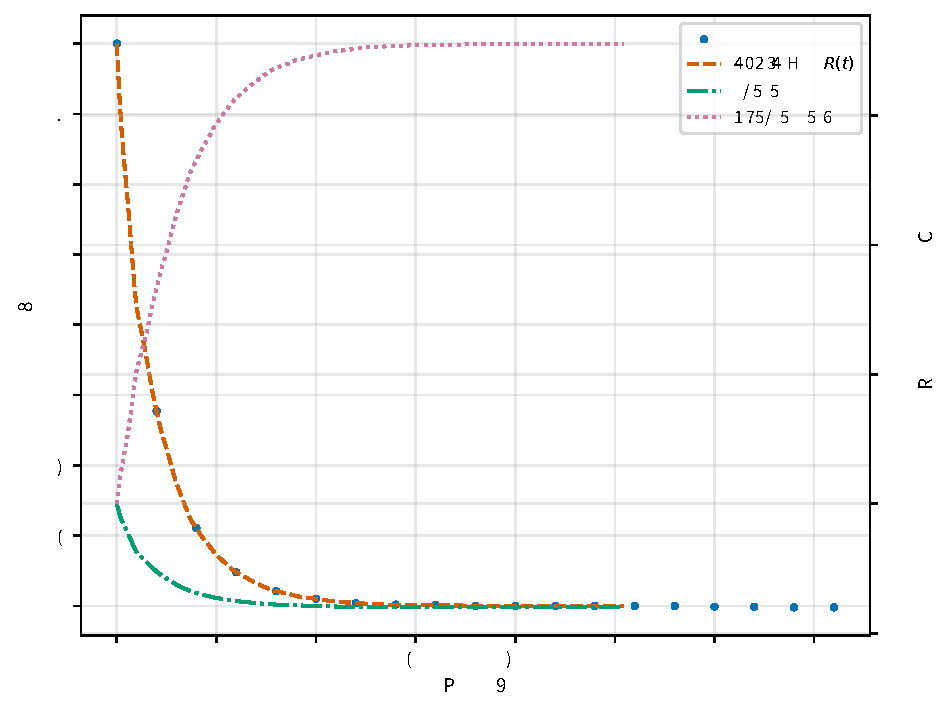
\includegraphics[width=0.78\textwidth]{figures/q4_shrinkage_scale}
  \caption{实测半径、收缩比与几何扩散尺度}
  \label{fig:q4-scale}
\end{figure}

\begin{figure}[htbp]
  \centering
  \begin{minipage}{0.48\textwidth}
    \centering
    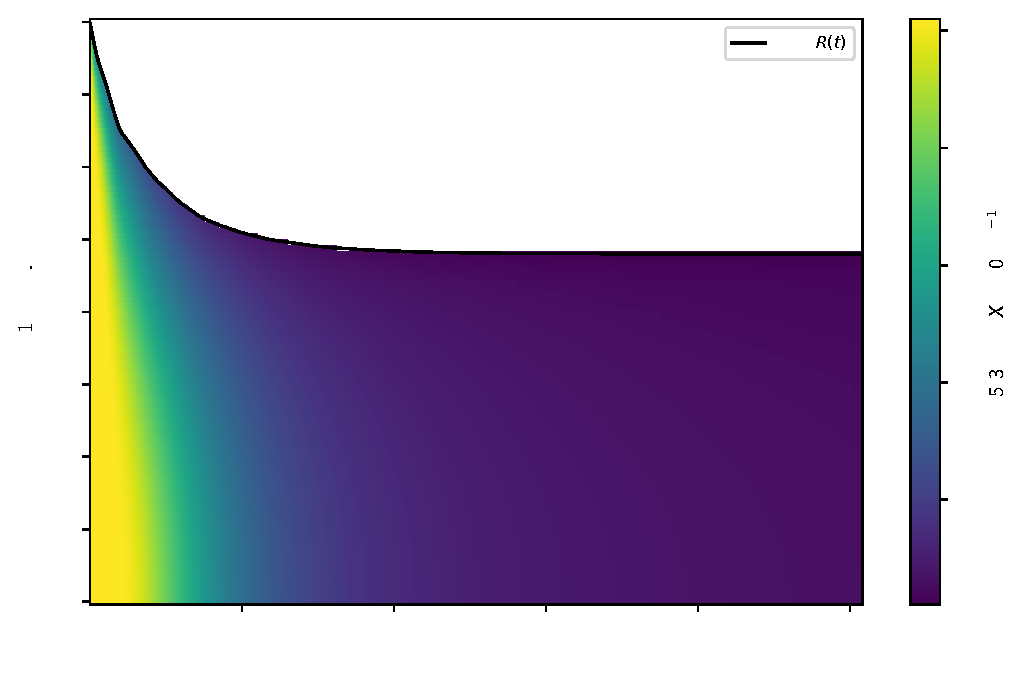
\includegraphics[width=\textwidth]{figures/q4_physical_heatmap}
  \end{minipage}
  \hfill
  \begin{minipage}{0.48\textwidth}
    \centering
    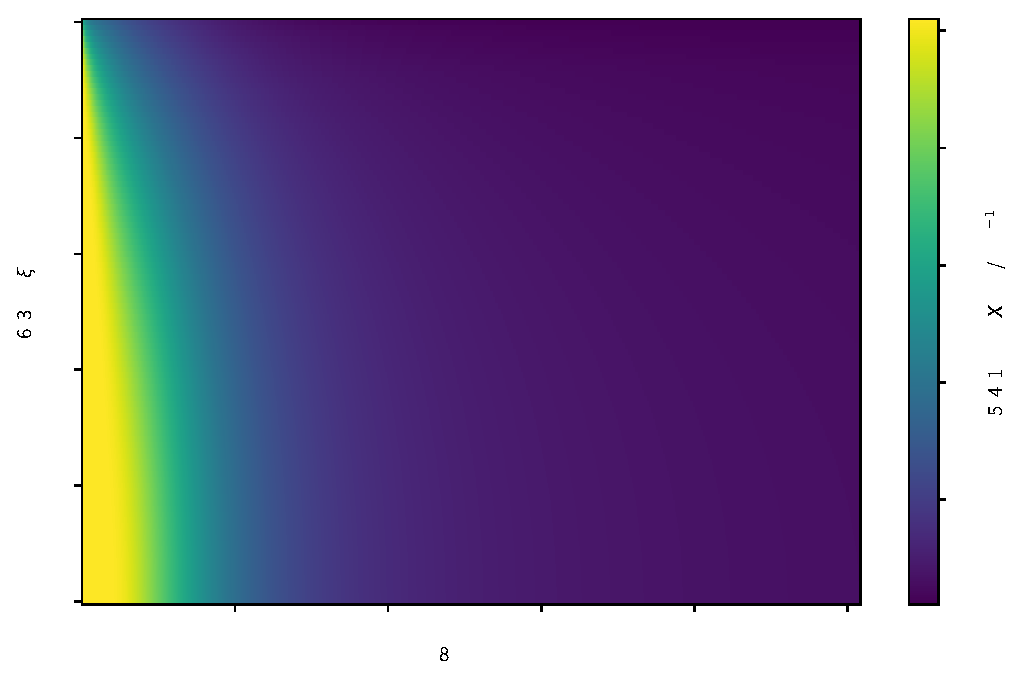
\includegraphics[width=\textwidth]{figures/q4_material_heatmap}
  \end{minipage}
  \caption{收缩工况含水率场：物理坐标（左）与材料坐标（右）。物理坐标
  图中的空白区域为收缩后位于药材外部的位置；两图均由正式 $0.1\ \mathrm{cm}$ 物理采样结果重构，用于描述宏观分布，不等同于原始 $321$ 单元求解场}
  \label{fig:q4-field}
\end{figure}

\begin{figure}[htbp]
  \centering
  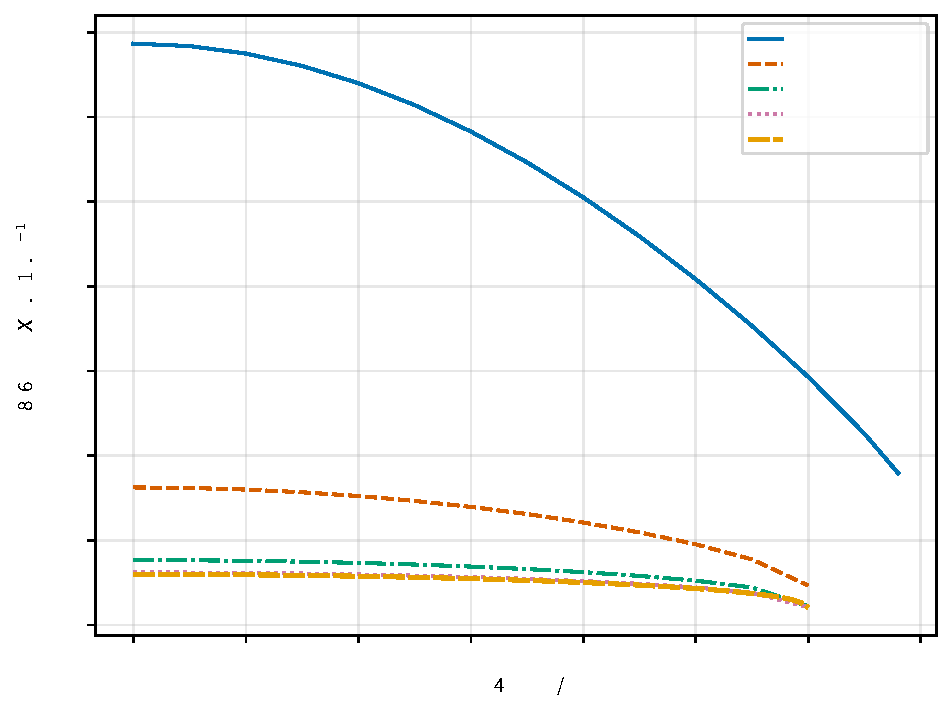
\includegraphics[width=0.82\textwidth]{figures/q4_profiles}
  \caption{收缩工况不同时刻的含水率径向剖面}
  \label{fig:q4-profiles}
\end{figure}

% 自动生成：python paper/build_tables.py（勿手工编辑）
\begin{table}[htbp]
\centering
\caption{收缩工况代表性时刻的干基含水率（单位：$\mathrm{kg\,kg^{-1}}$）}
\label{tab:t6}
\begin{tabular}{lccccc}
\toprule
时间/h & 0 cm & 0.5 cm & 1 cm & 1.5 cm & 药材表面 \\
\midrule
0 & 2.5500 & 2.5500 & 2.5500 & 2.5500 & 2.5500 \\
6 & 1.7164 & 1.5350 & 1.0212 &  & 0.4215 \\
12 & 0.7340 & 0.6516 & 0.4068 &  & 0.1666 \\
18 & 0.4065 & 0.3667 & 0.2387 &  & 0.0888 \\
24 & 0.2837 & 0.2598 & 0.1783 &  & 0.0671 \\
30 & 0.2253 & 0.2085 & 0.1488 &  & 0.0593 \\
36 & 0.1920 & 0.1790 & 0.1313 &  & 0.0558 \\
42 & 0.1706 & 0.1598 & 0.1196 &  & 0.0539 \\
48 & 0.1556 & 0.1463 & 0.1113 &  & 0.0529 \\
烘干结束时间（50.8235 h） & 0.1500 & 0.1413 & 0.1081 &  & 0.0525 \\
\bottomrule
\end{tabular}
\parbox{0.88\linewidth}{\footnotesize\textit{注：}表中每 6 h 取样；0--1.5 cm 为固定物理坐标，空白表示该位置已位于收缩后药材外部；“药材表面”为移动坐标 $r=R(t)$。末行为连续事件定位得到的精确烘干终止时刻。}
\end{table}


采用移动边界模型计算得到考虑收缩效应时的烘干终止时间为：

\begin{equation}
  t_{\mathrm{dry}}^{(4)}=182964.7\ \mathrm{s}=50.8235\ \mathrm{h},
  \label{eq:tdry4}
\end{equation}

相较固定半径工况，终止时间相差
$57.1904-50.8235=6.37\ \mathrm{h}$；但两工况分别采用附录 3 和附录
4 的经验物性关系，该差异不能直接归因于几何收缩。在终止时刻，中心区域含水率为
$0.1500\ \mathrm{kg\,kg^{-1}}$，满足干燥终止判据；表面含水率进一步
降低至 $0.0525\ \mathrm{kg\,kg^{-1}}$。不同时间下的径向含水率分布
如图 \ref{fig:q4-profiles} 所示。随着半径逐渐收缩，含水率分布曲线对应
的空间位置整体向内移动，超出实际材料范围的区域不再参与计算。

需要指出的是，固定半径工况与收缩工况分别采用附录 3 和附录 4 给出的
不同经验物性模型，因此两种情况下终止时间的差异不能完全归因于几何
收缩。为分离几何收缩效应，进一步采用附录 4 物性参数、但保持半径不变
的固定半径模型进行对照计算，得到终止时间
$464785.2\ \mathrm{s}=129.11\ \mathrm{h}$。由此可见，在相同物性条件
下，引入收缩后终止时间由 $129.11\ \mathrm{h}$ 降低至
$50.82\ \mathrm{h}$，缩短约 $60\%$，说明几何收缩对干燥过程具有显著
的促进作用。

收缩加速干燥主要体现在两个方面：

（1）缩短内部扩散距离。水分由内部向表面的迁移特征时间满足
$\tau_D\sim R^2/D_{\mathrm{eff}}$，而收缩使特征长度 $R$ 由 $2.00\ \mathrm{cm}$ 降至 $1.198\ \mathrm{cm}$（降低约 $40\%$），对应的 $R^2$ 降低约 $64\%$，因此显著缩短水分迁移所需时间。

（2）增大单位体积对应的表面积。圆柱侧表面积与体积之比为 $2/R$。在本
文的经验有效扩散模型中，这会增大单位体积对应的表面有效交换能力；随着
半径减小，该比例增大约 $67\%$，从而进一步促进内部水分向外迁移。

上述两种机制共同作用，使考虑收缩后的模型表现出更快的干燥过程，也验证
了移动边界模型在描述实际药材干燥行为中的必要性。

% ==================== 七、模型验证 ====================
\section{模型验证}

\subsection{解析基准验证}

问题一在常物性条件下可退化为经典圆柱坐标系下一维径向非稳态导热问题。
为验证所建立数值模型的准确性，选取恒定环境温度
$T_a=50\ ^\circ\mathrm{C}$ 条件下的 Robin 边界圆柱导热问题作为解析
基准。该问题存在基于 Bessel 函数展开的半解析解：

\begin{equation}
  T(r,t)=T_a+\sum_{n=1}^{\infty}A_n\,J_0\!\left(\frac{\lambda_n r}{R_0}
  \right)\mathrm{e}^{-\alpha_1\lambda_n^2 t/R_0^2},\qquad
  A_n=\frac{2(T_0-T_a)J_1(\lambda_n)}
  {\lambda_n\left[J_0^2(\lambda_n)+J_1^2(\lambda_n)\right]},
  \label{eq:bessel}
\end{equation}

其中，$\lambda_n$ 为 $\lambda J_1(\lambda)=\mathrm{Bi}\,J_0(\lambda)$
的正根。对于实际烘房温度随时间变化的情况，引入 Duhamel 叠加原理，将
变温边界条件转换为分段恒温响应的线性组合，构造对应的参考解。

计算中取空间网格数 $N=81$，并保留前 $300$ 阶特征模态进行比较。数值
结果与半解析解的最大温度偏差见表 \ref{tab:bessel}，误差均不超过
$0.04\ ^\circ\mathrm{C}$，约占整体温升幅度（约 $22\ ^\circ\mathrm{C}$）
的 $0.2\%$。结果表明，所建立模型能够准确捕捉 Robin 边界条件下圆柱体
内部温度演化过程，验证了有限体积离散、边界通量处理以及时间积分方法
的正确性。

\begin{table}[htbp]
  \centering
  \setcounter{table}{7}
  \caption{Q1 温度场与半解析参考解的最大偏差（$N=81$，单位：$^\circ\mathrm{C}$）}
  \label{tab:bessel}
  \begin{tabular}{lccc}
  \toprule
  参考解 & $t=60\ \mathrm{s}$ & $t=300\ \mathrm{s}$ & $t=1800\ \mathrm{s}$ \\
  \midrule
  Bessel（常 $T_a$） & $2.217\times10^{-2}$ & $3.882\times10^{-2}$ &
  $7.250\times10^{-3}$ \\
  Duhamel（时变 $T_a$） & $2.029\times10^{-4}$ & $4.157\times10^{-3}$ &
  $3.761\times10^{-3}$ \\
  \bottomrule
  \end{tabular}
\end{table}

上述偏差是数值解相对于已知参考解的离散误差，而非对实测内部温湿场的
预测残差。附件仅提供烘房环境与收缩半径序列，未提供可配对的
$T_{\mathrm{obs}}(r,t)$、$X_{\mathrm{obs}}(r,t)$；因此本文不虚构
$R^2$、RMSE 或置信区间，而以解析基准、收敛性与守恒型闭合构成当前数据
条件下可复现的数值验证链。若取得内部测温、含水率观测，才可在独立留出
数据上报告相应的预测误差。

\subsection{空间与时间收敛性}

为检验数值结果对空间网格与时间步长的敏感性，分别以烘干终止时间
$t_{\mathrm{dry}}$ 与公共时刻场值误差作为评价指标，开展空间与时间收敛
性分析，结果见表 \ref{tab:conv} 和图 \ref{fig:conv}。

在空间离散方面，将径向网格数由 $161$ 逐步加密至 $321$ 和 $641$。随着
网格加密，两种工况下的终止时间变化幅度逐渐减小：固定半径工况由
$149.56\ \mathrm{s}$ 降至 $52.59\ \mathrm{s}$；收缩工况由
$25.87\ \mathrm{s}$ 降至 $7.54\ \mathrm{s}$。同时，各加密层级之间的
场值差异降低至 $10^{-5}\sim10^{-4}$ 量级，表明空间离散误差已基本
收敛，计算结果具有稳定性。

在时间离散方面，将最大时间步长由 $60\ \mathrm{s}$ 逐渐减小至
$15\ \mathrm{s}$ 进行比较。结果显示，在固定半径和收缩工况下，终止
时间变化分别仅为 $0.26\ \mathrm{s}$ 和 $0.12\ \mathrm{s}$，明显小于
空间网格加密所引起的终止时间差异。因而在当前计算配置下，终止时间的
离散不确定性主要来自空间离散；连续事件二分的 $0.01\ \mathrm{s}$ 容差
只控制事件求根精度，不能代替 PDE 离散误差。

需要说明的是，连续事件定位方法用于保证终止时刻输出的一致性，并不意味
着模型具有超过设定离散精度的物理预测能力。最终结果保留四位小数，仅
依据题目要求进行输出。

\begin{table}[htbp]
  \centering
  \setcounter{table}{8}
  \caption{终止时间的空间网格收敛}
  \label{tab:conv}
  \begin{tabular}{lcccc}
  \toprule
  工况 & 网格变化 & $\Delta t_{\mathrm{dry}}$ / s &
  $\max|\Delta T|$ / $^\circ\mathrm{C}$ & $\max|\Delta X|$ \\
  \midrule
  固定半径 & $161\rightarrow321$ & $-149.56$ &
  $2.329\times10^{-5}$ & $2.183\times10^{-4}$ \\
  固定半径 & $321\rightarrow641$ & $-52.59$ &
  $5.866\times10^{-6}$ & $8.154\times10^{-5}$ \\
  实测收缩 & $161\rightarrow321$ & $-25.87$ &
  $6.617\times10^{-5}$ & $1.780\times10^{-4}$ \\
  实测收缩 & $321\rightarrow641$ & $-7.54$ &
  $1.664\times10^{-5}$ & $4.471\times10^{-5}$ \\
  \bottomrule
  \end{tabular}
\end{table}

\begin{figure}[htbp]
  \centering
  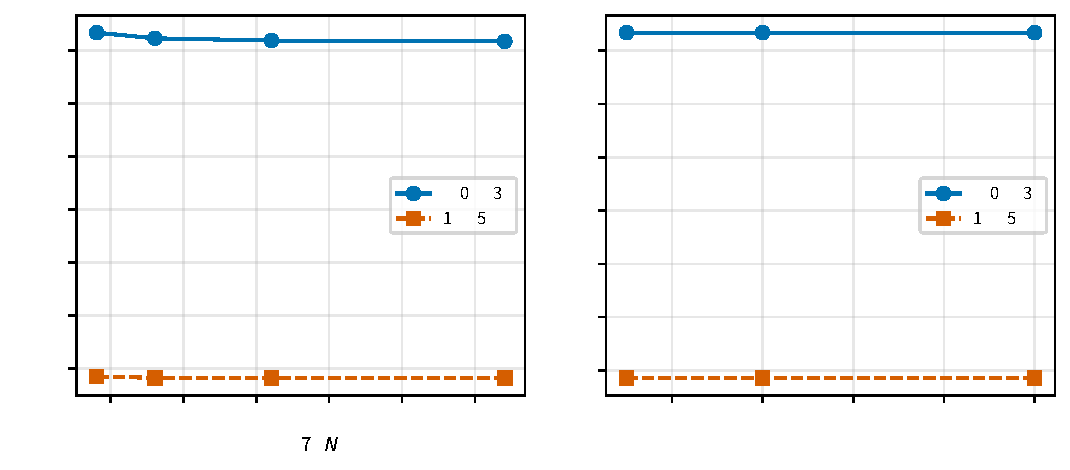
\includegraphics[width=0.82\textwidth]{figures/convergence}
  \caption{终止时间的空间网格与时间步收敛}
  \label{fig:conv}
\end{figure}

\subsection{积分通量闭合}

为检验水分迁移方程离散求解的通量一致性，对经验有效扩散方程在整个计算
域内积分，得到平均含水率变化与边界有效通量之间应满足的积分闭合关系：

\begin{equation}
  \bar X(t)-\bar X(0)
  +\int_0^t\frac{2h_m}{R(\tau)}
  \left[X_s(\tau)-\chi_a(\tau)\right]\,\mathrm d\tau=0.
  \label{eq:fluxid}
\end{equation}

其中，第一项表示计算域内平均含水率变化，第二项表示通过表面的累计水分
迁移量。

在网格数 $N=81$ 条件下，对 $0$--$12\ \mathrm{h}$ 完整时间区间进行
通量闭合检查。其中时间积分采用梯形积分，共包含 $1440$ 个积分区间；同时，
对干燥初期水分变化较快阶段进行加密检查，前 $4\ \mathrm{h}$ 共
$480$ 个时间区间均参与误差评估。结果表明，固定半径工况与收缩工况下，
相对 $12\ \mathrm{h}$ 总失水量的最大累计闭合误差分别为 $1.191\times10^{-5}$ 和
$1.298\times10^{-5}$（对应绝对闭合误差 $2.638\times10^{-5}$ 和 $2.695\times10^{-5}\ \mathrm{kg\,kg^{-1}}$）。该误差水平较小，说明离散计算过程中边界水分
通量、内部扩散过程以及平均含水率变化能够保持良好的数值一致性，验证了
经验有效扩散方程离散格式的通量闭合性与可靠性。该检查不等同于设备尺度
的严格水分质量守恒验证。

\subsection{物理约束与输出核对}

为进一步检验模型计算过程中的物理合理性，对全干燥过程进行物理约束
检查。取空间网格数 $N=81$，计算结果显示，两种工况下全域含水率始终
满足 $X_{\min}=0.0525\ge0$，且材料物性参数始终满足 $k>0$、
$D_{\mathrm{eff}}>0$。同时，药材内部温度始终处于环境温度范围
$28\ ^\circ\mathrm{C}\le T\le50.165\ ^\circ\mathrm{C}$，含水率径向
分布保持单调性，未出现非物理振荡现象，说明模型求解过程满足基本物理
约束。

进一步对长时间热场稳定性进行检验。结果表明，干燥 $24\ \mathrm{h}$
后全场温度与烘房环境温度的最大偏差为 $3.41\times10^{-13}\ ^\circ\mathrm{C}$
（收缩工况 $2.13\times10^{-13}\ ^\circ\mathrm{C}$），表明热场已达到稳定状态。
此外，将模型中的热传递项简化为 $T\equiv T_a$ 进行降阶模型对比，终止
时间分别缩短 $308.9\ \mathrm{s}$（固定半径）和 $283.2\ \mathrm{s}$（收缩工况）。两者相对于完整模型
终止时间的变化均小于 $0.2\%$。因此，长时间干燥阶段热场耦合对最终烘干
时间影响较小，模型输出结果具有较好的稳定性与可信度。

\subsubsection*{环境水分势排序诊断与输出核对}

对长期平台水分势 $C_a=0.03,\ 0.05,\ 0.07$ 作排序诊断，终止时间随空间
网格的变化为：$N=81$ 对应 $207397.3$、$206420.9$、$208191.2\ \mathrm{s}$；
$N=161$ 对应 $206039.7$、$206041.6$、$208125.0\ \mathrm{s}$；
$N=321$ 对应 $205351.5$、$205894.0$、$208106.1\ \mathrm{s}$。仅在
$N=321$ 上终止时间随 $C_a$ 单调递增：$N=81$ 的 $0.03$ 与 $0.05$ 两项
顺序相反（$207397.3>206420.9$），$N=161$ 的这两项又几乎重合（相差约
$2\ \mathrm{s}$）；$0.05\to0.07$ 的排序在三个网格上一致。由于
$D_{\mathrm{eff}}$ 随 $X$ 迅速下降，较低 $C_a$ 可能先形成低扩散率的干燥
表层，在网格收敛前不宜把 $N=321$ 的单调性解释为已确证的真实机理。作为
边界符号与实现的独立对照，固定扩散系数
$D=3.6\times10^{-9}\ \mathrm{m^2\,s^{-1}}$ 的控制组给出 $100920.0$、
$105843.6$、$112020.0\ \mathrm{s}$，在三个 $C_a$ 水平上严格单调，说明
边界符号与数据流方向正确。

针对问题一初始边界层的数值收敛性进行了专项检验。表面含水率在
$t=1\ \mathrm{s}$ 时，随着空间网格由 $N=641\to1281\to2561$ 逐步加密，
计算结果由 $2.5173\to2.5176\to2.5177$ 收敛；同时，将初始时间步由
$0.25\ \mathrm{s}\to0.015625\ \mathrm{s}$ 细化后，结果收敛至
$2.5177$。说明初始阶段极薄水分边界层已得到充分解析，四位小数精度
满足要求。此外，在 $t=1800\ \mathrm{s}$ 时，采用不同空间网格 $N=161$
与 $N=641$ 计算得到表面含水率均为
$1.5102\ \mathrm{kg\,kg^{-1}}$，进一步验证了长期计算
结果的空间稳定性。

最后，对正式输出结果进行逐项核对。四个工作簿中的时间网格、径向采样
网格、四舍五入规则以及越界空值标记均符合题目要求。表 1--6 均由冻结
计算结果自动生成，并与
\texttt{result1.xlsx}--\texttt{result4.xlsx} 中的数值保持一致。

% ==================== 八、灵敏度分析与工艺情景 ====================
\section{灵敏度分析与工艺情景}

\subsection{参数灵敏度}

为分析关键物性参数与环境条件对干燥过程的影响规律，选取终止时间
$t_{\mathrm{dry}}$ 作为评价指标，在空间网格数 $N=321$ 条件下，对主要
影响参数进行单因素扰动分析。通过改变各参数取值并保持其他条件不变，
比较不同参数水平下烘干终止时间的变化趋势，结果见表 \ref{tab:sens} 与
图 \ref{fig:sens}。

对于乘性扰动参数 $p\in\{h_T,h_m,C_a\}$，以有限差分弹性量化局部响应：
\begin{equation}
  S_p=\frac{[t_{\mathrm{dry}}(p)-t_0]/t_0}{(p-p_0)/p_0},
  \qquad t_0=205885.2\ \mathrm{s}.
  \label{eq:sensitivity}
\end{equation}
这里 $S_p$ 仅描述该给定基准附近、其余输入不变时的单因素响应；平台温度
采用绝对温差报告，不将摄氏温度不恰当地作百分比弹性处理。

\begin{table}[htbp]
  \centering
  \setcounter{table}{9}
  \caption{参数灵敏度（$N=321$ 重算基准 $t_{\mathrm{dry}}=205885.2\ \mathrm{s}$）}
  \label{tab:sens}
  \begin{tabular}{lcc}
  \toprule
  场景 & $t_{\mathrm{dry}}$ / s & $\Delta t_{\mathrm{dry}}$ / h \\
  \midrule
  $h_T\times0.8$ & $205956.5$ & $+0.020$ \\
  $h_T\times1.2$ & $205838.1$ & $-0.013$ \\
  $h_m\times0.5$ & $232696.6$ & $+7.45$ \\
  $h_m\times1.5$ & $198782.5$ & $-1.97$ \\
  $h_m\times2.0$ & $195865.9$ & $-2.78$ \\
  平台温度 $-2\ ^\circ\mathrm{C}$ & $219548.7$ & $+3.80$ \\
  平台温度 $+2\ ^\circ\mathrm{C}$ & $193390.3$ & $-3.47$ \\
  $C_a\times0.9$ & $205619.1$ & $-0.074$ \\
  $C_a\times1.1$ & $206244.3$ & $+0.100$ \\
  低温高湿联合情景 & $219893.3$ & $+3.89$ \\
  高温低湿联合情景 & $193106.2$ & $-3.55$ \\
  \bottomrule
  \end{tabular}
\end{table}

\begin{figure}[htbp]
  \centering
  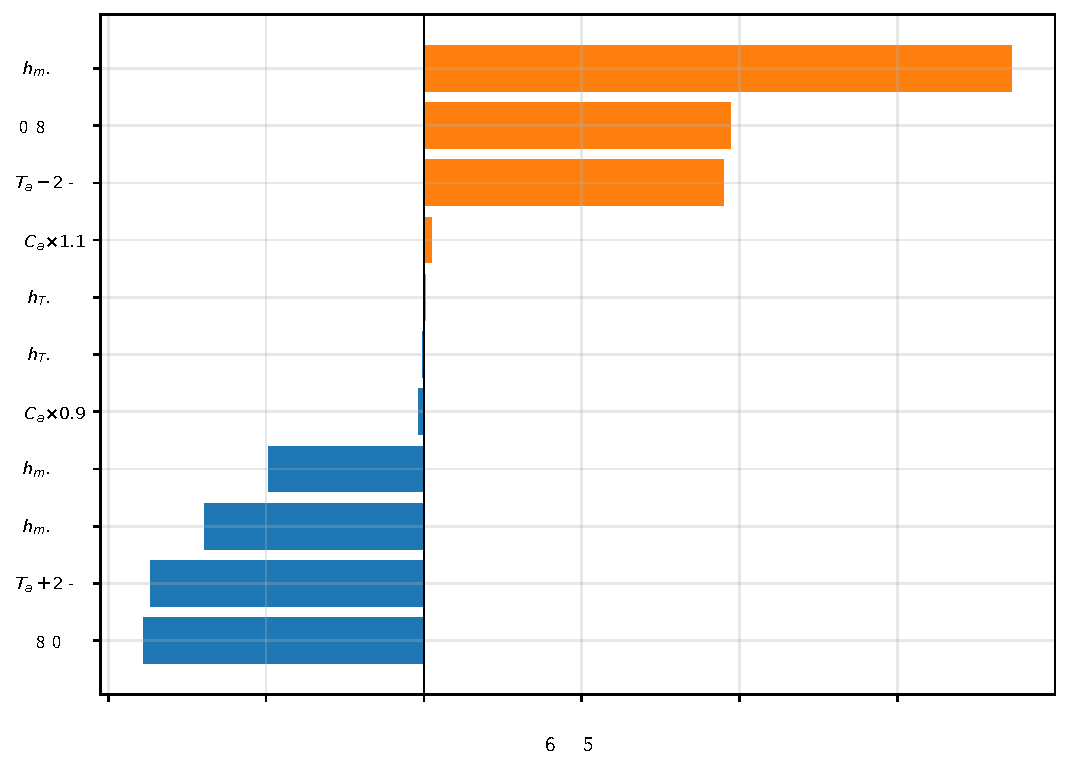
\includegraphics[width=0.76\textwidth]{figures/sensitivity}
  \caption{单因素及边界联合情景对终止时间的影响（龙卷风图）}
  \label{fig:sens}
\end{figure}

结论如下：

（1）终止时间对换热系数 $h_T$ 不敏感。在 $\pm20\%$ 扰动范围内，终止
时间仅变化 $-47.1$ 至 $+71.3\ \mathrm{s}$（$-0.023\%$ 至 $+0.035\%$），
对应 $|S_{h_T}|\le 1.73\times10^{-3}$。这与预热阶段占整个干燥过程比例
较小、且恒温阶段热场趋于稳定的数值结果一致。

（2）传质系数 $h_m$ 是影响终止时间的主要敏感参数。减小 $h_m$ 会使终止
时间延长约 $7.45\ \mathrm{h}$（约 $13.0\%$），而增大 $h_m$ 至两倍可使
干燥时间缩短约 $2.78\ \mathrm{h}$。相应 $|S_{h_m}|$ 为
$0.049$--$0.260$，远高于 $h_T$；这说明基准闭合中传质系数的不确定性
应优先控制，但不将该局部灵敏度直接等同于未观测的真实传质阻力占比。

（3）恒温阶段环境温度对干燥时间具有明显影响。温度每升高
$2\ ^\circ\mathrm{C}$，终止时间约缩短 $3.5$--$3.8\ \mathrm{h}$，其
主要原因在于温度升高通过 Arrhenius 关系
$\exp(-3850/\Theta)$ 增强有效扩散系数，加快药材内部水分迁移。

（4）环境水分势 $C_a$ 对终止时间影响较弱。在 $\pm10\%$ 扰动范围内，
终止时间变化为 $-0.074$ 至 $+0.100\ \mathrm{h}$，对应
$|S_{C_a}|=0.013$--$0.017$。联合的低温高湿、高温低湿边界情景分别使
终止时间相对基准增加 $3.89\ \mathrm{h}$、缩短 $3.55\ \mathrm{h}$，且均
得到连续事件时刻。该有界情景检验考察的是边界闭合扰动下的数值响应，并非
不适用于本题 PDE 的随机可行解或全局最优性证明。

\subsection{平台温度情景与终点均匀性}

实际干燥工艺中需要关注的不仅是缩短干燥时间，还需保证终点含水率分布
均匀。因此，在保持前 $4\ \mathrm{h}$ 实测升温过程不变的基础上，仅改变
恒温阶段的平台温度设定值，开展平台温度情景分析。在
$48$--$52\ ^\circ\mathrm{C}$ 范围内以 $0.25\ ^\circ\mathrm{C}$ 为步长取
$17$ 个均匀温度点，再插入实测平台 $50.165\ ^\circ\mathrm{C}$，共
$18$ 组工况（空间网格取 $N=321$，并采用 $N=641$ 进行抽查验证），以烘干终止时间 $t_f$ 和终点截面含水率加权标准差 $\sigma_X$
作为评价指标：

\begin{equation}
  \sigma_X(t_f)=
  \left[\frac{2}{R^2}\int_0^R\left(X-\bar X\right)^2r\,\mathrm dr
  \right]^{1/2}.
  \label{eq:sigma}
\end{equation}

\begin{figure}[htbp]
  \centering
  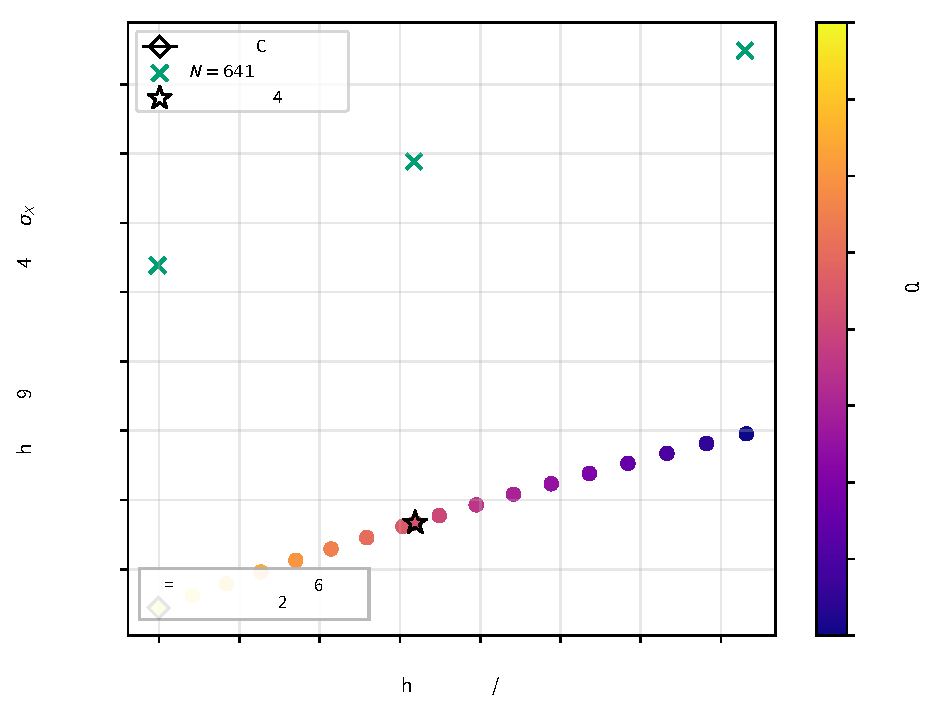
\includegraphics[width=0.82\textwidth]{figures/pareto_time_uniformity}
  \caption{终止时间—终点含水率均匀性目标空间（颜色为平台温度，
  黑色菱形为非支配集合）}
  \label{fig:pareto}
\end{figure}

计算结果如图 \ref{fig:pareto} 所示。随着平台温度由实测值
$50.165\ ^\circ\mathrm{C}$ 提高至 $52\ ^\circ\mathrm{C}$，终止时间由
$57.1904\ \mathrm{h}$ 缩短至 $53.9942\ \mathrm{h}$，减少
$3.1962\ \mathrm{h}$（约 $5.59\%$）；当温度降低至
$48\ ^\circ\mathrm{C}$ 时，终止时间延长至 $61.31\ \mathrm{h}$。与此
同时，终点含水率均匀性指标 $\sigma_X$ 随温度变化仅轻微下降
（由实测平台 $50.165\ ^\circ\mathrm{C}$ 的 $0.0194273$ 变为 $52\ ^\circ\mathrm{C}$ 的 $0.0194249$，变化量仅 $2.45\times10^{-6}$）。而
$N=321$ 与 $N=641$ 两种网格计算结果的最大差异为 $1.106\times10^{-5}$，
约为温度引起变化幅度的 $4.51$ 倍。因此，在当前空间离散精度下，平台
温度对终点均匀性的影响尚不可分辨。

综合来看，提高平台温度能够明显缩短干燥终止时间，而未观察到终点含水率
均匀性的明显恶化。由于研究区间内两个评价指标不存在可分辨的竞争关系，
本文将 $52\ ^\circ\mathrm{C}$ 作为给定温度范围内的优选工艺方案，而非
超出模型假设范围的全局最优温度。

需要指出的是，该结论具有明确的适用范围。模型未考虑有效成分热降解、
色泽变化、挥发性成分损失、组织损伤以及设备能耗等因素，因此不能据此推断
实际生产中的全局最优温度。此外，温度情景分析基于固定几何模型，受限于
现有实测收缩曲线，无法进一步确定不同平台温度下的
$R(t;T_{\mathrm{plat}})$ 变化规律。

% ==================== 九、模型评价、局限与推广 ====================
\section{模型评价、局限与推广}

\subsection{模型优势与证据}

\textbf{统一求解结构处理了四问中不变的守恒骨架与变化的物性、几何。}
固定域和材料坐标域均采用单元中心有限体积通量、半单元 Robin 阻力与
Backward Euler--BDF2 时间推进；问题间只替换物性、半径输入和输出契约。
这使问题 3 的全域阈值与问题 4 的实测收缩能够在同一连续事件框架下处理，
所得终止时刻分别为 $57.1904\ \mathrm{h}$ 和 $50.8235\ \mathrm{h}$，而非由
$60\ \mathrm{s}$ 表格节点近似。特别地，问题 4 将厘米级实测半径以 PCHIP 映射
到材料坐标，并在 $241200\ \mathrm{s}$ 后钳制为 $0.01198\ \mathrm{m}$，避免了
移动域插值在平台段产生非物理超调。

\textbf{离散格式与交付结果具有可追溯的数值检验链。}
Q1 热方程相对 Bessel/Duhamel 参考解的最大温度偏差不超过
$0.04\ ^\circ\mathrm{C}$；$N=321\to641$ 时，固定半径和收缩工况的终止
时间分别仅改变 $52.59\ \mathrm{s}$ 和 $7.54\ \mathrm{s}$；水分通量闭合的最大
累计误差为 $1.191\times10^{-5}$、$1.298\times10^{-5}$。这些检验分别对应
方程/边界离散、空间分辨率及通量一致性，而工作簿审计再将表 1--6 与冻结
轨迹、连续事件行逐项核对，避免把输出采样精度误作物理预测精度。

\textbf{工艺比较保留了结论的可辨识边界。}
对 $h_T,h_m,C_a$ 和平台条件的有界扰动表明，$h_m$ 减半使终止时间延长
$7.45\ \mathrm{h}$，是应优先控制的边界闭合不确定性；平台温度由
$50.165$ 升至 $52\ ^\circ\mathrm{C}$ 则缩短 $3.1962\ \mathrm{h}$。但终点
均匀性温度信号仅为网格差的 $1/4.51$，故本文只报告“未观察到可分辨的
均匀性恶化”，并把 $52\ ^\circ\mathrm{C}$ 限定为考察区间内的条件优选，
不宣称生产全局最优。

\subsection{适用边界与对应改进}

\begin{table}[H]
  \centering
  \setcounter{table}{10}
  \caption{模型适用边界及可验证的后续改进路径}
  \label{tab:limits}
  \begin{tabularx}{\textwidth}{p{0.23\textwidth}X}
  \toprule
  当前限制及其影响 & 对应的改进路径 \\
  \midrule
  水分以 $D_{\mathrm{eff}}(X,\Theta)$ 的经验有效扩散闭合；现有附件没有
  内部 $T(r,t)$、$X(r,t)$ 观测，故不能识别液水、蒸气和相变项，也不能以
  $R^2$ 或 RMSE 声称预测精度。 & 设计独立的内部测温、分层含水率试验；在留出
  工况上标定并检验多相多孔介质模型及潜热闭合，而不是用同一 PDE 模拟标签
  训练替代模型。 \\
  一维轴对称域忽略端部传递、轴向收缩和样品间遮挡；常数 $h_T,h_m$ 也未
  描述风速、表面状态随时间的变化。 & 对具有端部效应或非均匀送风的设备，采集流场和
  多位置温湿度后扩展为二维轴对称/三维模型，并建立 $h_T,h_m$ 对风速与表面
  状态的受试验约束关联。 \\
  $R(t)$ 是附件 2 在单一过程下的直接几何输入；因此平台温度扫描保持固定
  几何，不能预测 $R(t;T_{\mathrm{plat}})$。 & 在多个平台温度下重复测量半径，拟合并交叉验证
  收缩--含水率--温度本构关系；再将其耦合到材料坐标方程。 \\
  优化指标只含终止时间和终点含水率离散度，未输入能耗、有效成分降解、
  色泽或组织损伤数据。 & 补充设备功率、品质动力学和产品检测数据；在这些
  可观测目标上构造多目标帕累托决策，而非把当前 $52\ ^\circ\mathrm{C}$ 的条件比较
  外推为最优生产配方。 \\
  Q1 为解析 $t=1\ \mathrm{s}$ 强边界层使用 $N=2561$、
  $\Delta t_{\max}=0.03125\ \mathrm{s}$；长时高分辨率计算成本随网格和时间层数增加。 & 在保持守恒通量与网格收敛检验的前提下，采用
  边界层自适应网格或并行三对角批处理；任何加速方案均须重新比较事件时间和
  通量闭合误差。 \\
  \bottomrule
  \end{tabularx}
\end{table}

\subsection{可迁移的建模结构}

本文可推广的不是附录中的经验系数或本题数值，而是“\textbf{实测外部驱动 +
径向守恒扩散 + Robin 表面交换 + 连续阈值事件}”这一结构。对于根茎类药材、
果蔬圆柱切片、木材圆棒或多孔颗粒的热风脱水，只要几何近似轴对称且能够获得
各自的物性、环境序列与表面交换参数，便可替换 $k,D_{\mathrm{eff}},h_T,h_m$ 和
初始条件，沿用有限体积--事件定位流程求取温湿场及达到工艺阈值的时间。

在工业干燥设备中，该结构还可作为批次过程的离线工艺比较器：以记录的烘房
温湿度和抽样半径作为输入，比较不同平台策略对终止时间的影响；若增加内部
温湿度传感器，则可用独立观测校正模型参数并形成在线状态估计。对于球形或
平板样品，可将径向散度项替换为相应几何的守恒通量；对于显著端部传递、各向
异性或强收缩的对象，则必须采用上一节所述的二维/三维扩展，不能直接套用
本题一维结果。

% ==================== 参考文献 ====================
\begin{thebibliography}{99}

\bibitem{simal1998}
Simal S, Rossell\'o C, Berna A, et al. Drying of shrinking
cylinder-shaped bodies[J]. Journal of Food Engineering, 1998,
37(4): 423--435.

\bibitem{hussain2003}
Hussain M M, Dincer I. Two-dimensional heat and moisture transfer
analysis of a cylindrical moist object subjected to drying: A
finite-difference approach[J]. International Journal of Heat and
Mass Transfer, 2003, 46(21): 4033--4039.

\bibitem{tao2001}
陶文铨. 数值传热学[M]. 第2版. 西安: 西安交通大学出版社, 2001.

\bibitem{fritsch1980}
Fritsch F N, Carlson R E. Monotone piecewise cubic interpolation[J].
SIAM Journal on Numerical Analysis, 1980, 17(2): 238--246.

\bibitem{cumcm2026}
全国大学生数学建模竞赛组委会. 2026年高教社杯全国大学生数学建模竞赛
A题: 药材的烘干问题[EB/OL]. 2026.

\bibitem{crank1975}
Crank J. The Mathematics of Diffusion[M]. 2nd ed. Oxford: Clarendon Press,
1975.

\bibitem{patankar1980}
Patankar S V. Numerical Heat Transfer and Fluid Flow[M]. Washington, DC:
Hemisphere Publishing, 1980.

\bibitem{gear1971}
Gear C W. Numerical Initial Value Problems in Ordinary Differential
Equations[M]. Englewood Cliffs, NJ: Prentice-Hall, 1971.

\bibitem{virtanen2020}
Virtanen P, Gommers R, Oliphant T E, et al. SciPy 1.0: fundamental algorithms
for scientific computing in Python[J]. Nature Methods, 2020, 17(3): 261--272.
DOI: 10.1038/s41592-019-0686-2.

\bibitem{mujumdar2014}
Mujumdar A S, ed. Handbook of Industrial Drying[M]. 4th ed. Boca Raton:
CRC Press, 2014.

\end{thebibliography}

% ==================== 附录 ====================
\section*{附录 A \quad 正式输出文件说明}

\begin{table}[htbp]
  \centering
  \setcounter{table}{11}
  \caption{正式输出工作簿}
  \label{tab:app-out}
  \begin{tabular}{llccc}
  \toprule
  文件 & 内容 & 数据行 & 时间范围 / s & 时间间隔 / s \\
  \midrule
  \texttt{result1.xlsx} & 预热阶段温度与含水率 & $1800$ & $1$--$1800$ & $1$ \\
  \texttt{result2.xlsx} & 固定半径完整温度与含水率 & $205885$ &
  $1$--$205885$ & $1$ \\
  \texttt{result3.xlsx} & 固定半径含水率 & $3431$ & $60$--$205860$ & $60$ \\
  \texttt{result4.xlsx} & 收缩工况含水率 & $3049$ & $60$--$182940$ & $60$ \\
  \bottomrule
  \end{tabular}
\end{table}

精确终止事件及对应场保存在 \texttt{results/tables/} 目录中的 Q2、Q4
元数据文件。
\texttt{result3.xlsx} 与 \texttt{result4.xlsx} 仅保存严格早于连续终止
事件的规则 $60\ \mathrm{s}$ 时间点。

\section*{附录 B \quad 核心代码}

求解框架共两个核心模块：物性与环境输入（\texttt{props.py}）与统一有限
体积求解器（\texttt{solver.py}），完整代码附下。

\lstinputlisting[language=Python,
  caption={props.py：物性模型与环境/几何输入},
  label={lst:props}]{../src/props.py}

\lstinputlisting[language=Python,
  caption={solver.py：统一有限体积求解器（略去已注释的验证打印）},
  label={lst:solver}]{../src/solver.py}

\end{document}
